%\addcontentsline{toc}{chapter}{Software}
\section{Software}
\label{software}
 %%%%%%% INTRODUCTION %%%%%%
%%\addcontentsline{toc}{section}{Introduction}
%\section{Introduction}
In this section the software developed in this Bachelor's Thesis is presented and thoroughly explained. 
\\

The code was created as a ROS package. ROS (Robotic Operating System) is an Operating System designed to be implemented in robots. It has libraries to enhance the communication between nodes, the processes management or the threads present in the code among other functionalities. 
Since this code is intended to be running on a robot, the software developed was created as a ROS package. 
\\

In order to manage 2D and 3D information (images and point clouds) two libraries has been used: OpenCV, and PCL. Those two libraries implement basic and state-of-the-art algorithms that allow a easier and more time-efficient management of the data. Further information about these libraries might be found on the sections \ref{opencv} and \ref{pcl} respectively. 
\\

The software was structured in nodes. These nodes have a relatively small functionality and run in parallel. The fact that they run simultaneously improves the efficiency of the code lowering the lag due to time-expensive operations. 
\\

In the following sections, the software structure and tools used are described. 



%\section{Structure}
%\label{structure}

%In this section, the code functionalities of each part or node of the software are explained. The communication between nodes is shown and the overall software flow is thoroughly described. 

The code is structured in nodes. Each node contains a piece of the processing needed in the code. All nodes are related between them using ROS messages to transport the input and output data. 
\\

Computer vision is a field that involves high time-expensive algorithms. In the previous chapter it was explained that it uses 2D and 3D information. That information implies a matrix that has for each point 2 coordinates number (in the case of 2D) or 3 coordinates (in the case of 3D data), apart from the colour of that point, which is described using 3 more integers. \\

As it can be seen the data handled is enormous an the way to reduce the time lag due to those computations is modularizing the computation and executing in parallel those processes. 
\\

The software was designed to be as modular as was possible so that each node performs an action that could be used in other applications. 
As an example, the code could be easily changed to recognize hats or shoes, just changing the initial node that extracts the information of the desired joint. 
\\

In the following paragraphs the nodes' functionalities will be described and the communication between them presented. But first, the overall software work-flow is shown using the flow diagram below. 
\newpage

\subsection{Solution description}

The input of the system is the information coming from the RGB-D sensor. There are two different data that are taken: the 2D information, i.e. the raw image detected by the sensor's camera, and the 3D information, i.e. the raw point cloud. Also, there is another input to the system that shows the position of the different user's joints. This data is provided by a third-party package called pi\_tracker that is explained in the following chapters. 
\\

The software was designed to be running on a robot as was previously explained. This implies that there can not be a GUI (Graphical User Interface) on a screen because the robot being used might not have it. Also, the usability and easiness to learn how to interact with the program was important to allow different people not only investigators to use it. 
\\


\begin{figure}[H]
	\begin{center}
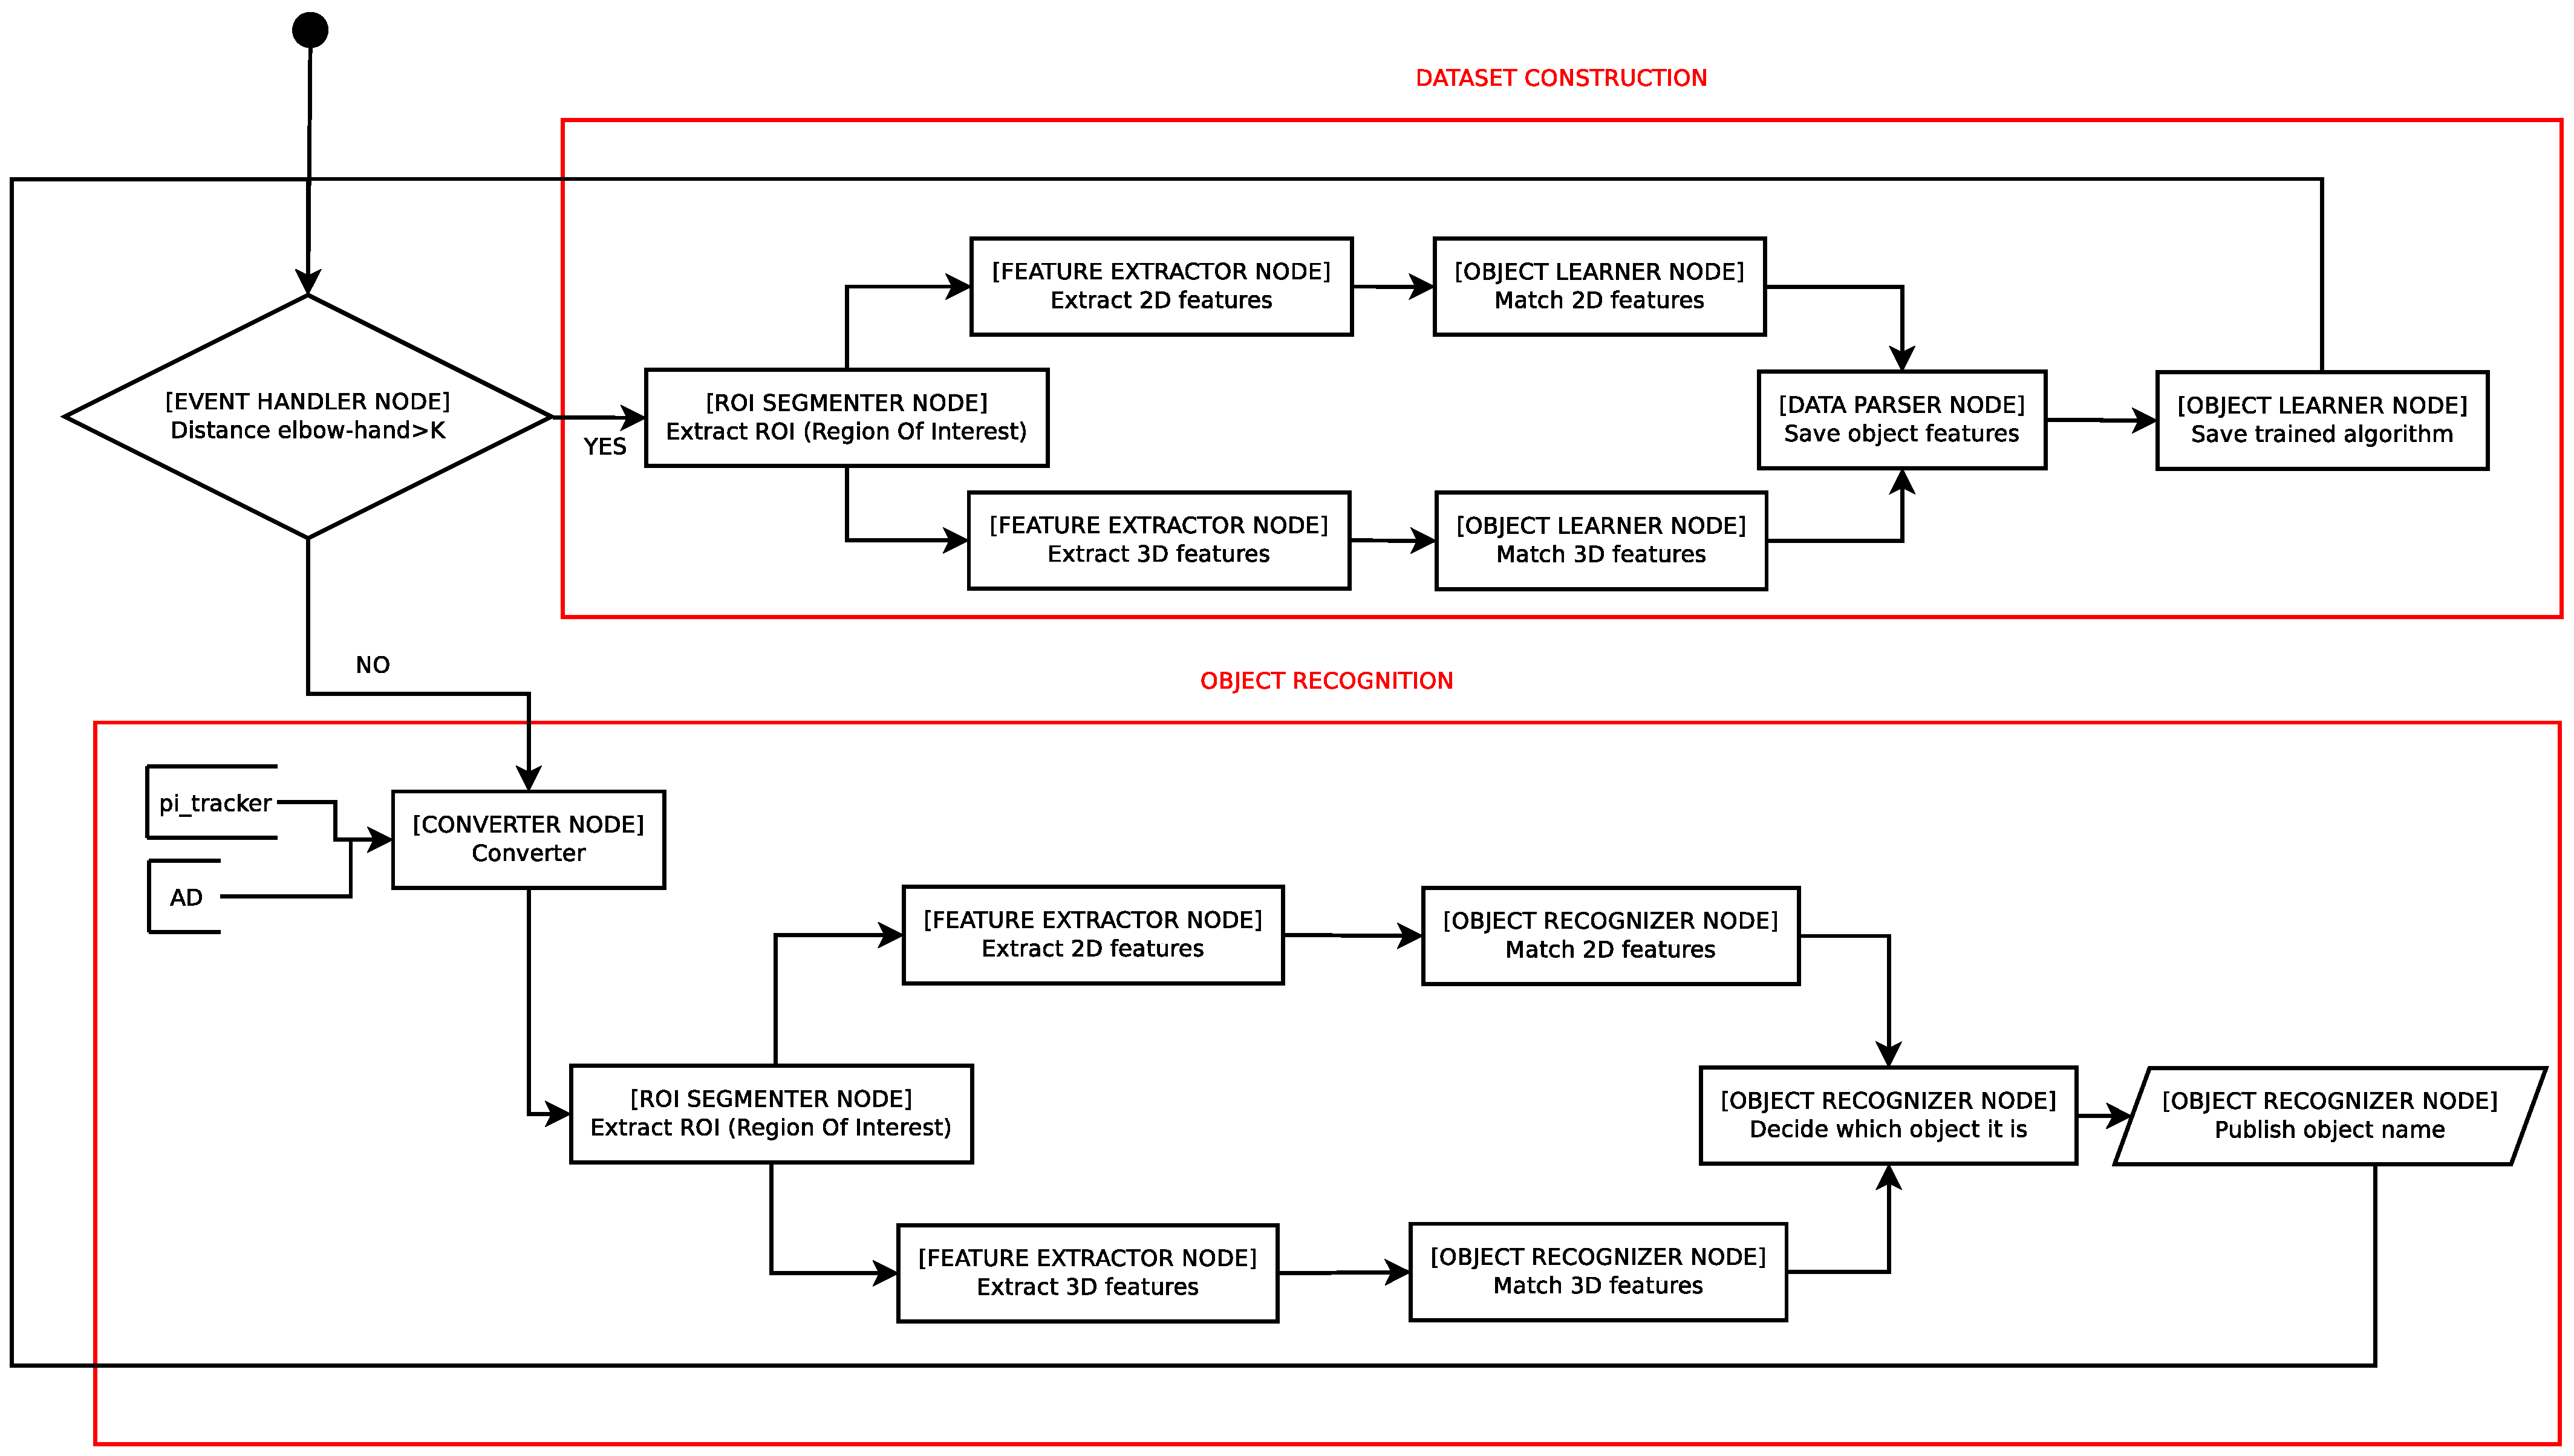
\includegraphics[scale=0.3]{img/diagrams/flowcharts.eps}
	\caption[Software flowchart]{Complete Software flowchart showing the different processing steps between the input and the output}
	\end{center}
\end{figure}


In order to fulfill those requirements a gestural interface was designed. It is developed by a separate node so the processing lags will not affect the recognition of the different gestures. This fact also allows an easy change of the gestures being used. 
\\

The recognition of the location of the hand with respect to the user's body shows how the arm is positioned. If it is stretched towards the sensor, the software enters the dataset construction mode, i.e. the data acquisition and learning mode. If, otherwise, it is located closer to the body, the software starts the object recognition mode. 
\\


The upper part of the diagram shows the data acquisition work-flow. The first step is to extract the ROI (Region of Interest) from the input raw data. This is a crucial step that allows to reduce noticeably the amount of time due to computation reducing the size of the processed information. 
\\

After the extraction, the 2D and 3D features of the segmented data are obtained. The features or descriptors are characteristics that define and represent the data from where they were created. There are different algorithms that perform this task with better or worse repeatability and robustness. All the details about this process is explained in the next chapters. 
\\

That is the end of the data cycle of the learning process. It is iterated over the number of views for each object that is required in order to obtain all the templates necessary per object. 
\\

The recognition mode was triggered when the hand was located near the user's body. This mode can be seen in the lower part of the previous diagram. 
\\

The steps that compose this part of the software are the following: 
First, the input information is converted to the custom message used within the code. Afterwards, as in the previous mode, the Region Of Interest is segmented from both 2D and 3D original information. Then, the descriptors are extracted exactly the same way as in the previous mode. 
\\

The next step is the recognition algorithm. This matches the descriptors from both the image and the point cloud and decides which object of the dataset is more similar to the one that is currently on the user's hand. More details about this algorithm may be found in this section. 
\\

Finally, the object identification number is obtained. This data is the output of the system. 


\newpage
\subsection{Third party libraries that process the input data to the system}
\label{ros_packages}
In this section the ROS packages that are used in our system are presented. 
All of them are used for the initial processing of the data coming from the RGB-D sensor. 
The connection between them and the developed nodes are explained in this section and in section \ref{nodes}.

\subsubsection{ROS package: openni\_camera}
\label{openni_camera}

This package implements the RGB-D sensors drivers.
% It is needed to connect the kinect to the computer. 
% The package is composed of nodes that perform different tasks and publish the results in topics. 
% As an example, a node transforms the raw output information of the kinect into a data array for further processing. 
The package transforms the input raw data coming from the kinect into structured one. 
This information is prepared hence for further processing. 
Figure \ref{diagram_kinect_data} shows the Connectivity graph of this package and its position in the RGB-D sensor data processing chain. 
 
 		\begin{figure}[H]
			\begin{center}
			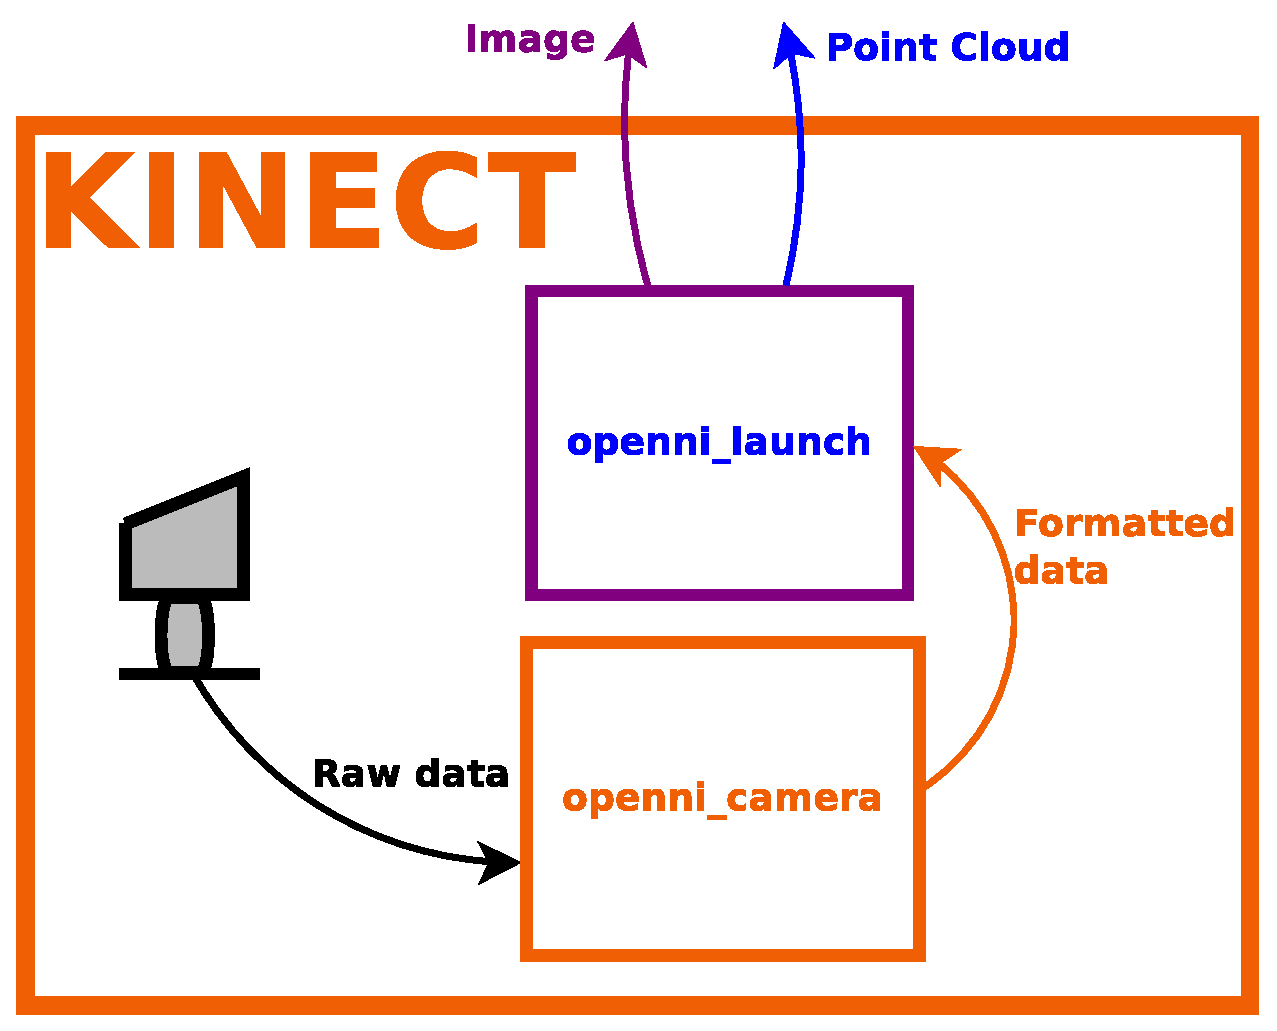
\includegraphics[width=0.5\linewidth]{img/diagrams/kinect_data.eps}
			\caption[Kinect data processing]{Kinect data processing using the openni ROS packages (openni\_camera and openni\_launch).}
			\label{diagram_kinect_data}
			\end{center}
		\end{figure}


\subsubsection{ROS package: openni\_launch}
\label{openni_launch}

This package provides useful transformations taking as input the openni\_camera topics. %and a launch file that executes nodelets with that information. 
It is composed of various nodes that can be executed using a launch file. 
Each node processes the raw input information from the driver into more useful data. 
This data may be a point cloud with color information or a disparity image for example. 
The output of the nodes is published into different topics. 
% The developed nodes described in section \ref{nodes} are subscribed to these topics in order to obtain the input point cloud and image. 
These topics are the input for the nodes that have been developed for this thesis.

\subsubsection{ROS package: pi\_tracker}

This ROS package implements a joint tracker.
It is used within the system to determine the position and orientation of the user's joints. 
This task is performed by the skeleton tracker node.  
Figure \ref{diagram_skeleton} shows the Connectivity graph of this node. 
% In figure \ref{diagram_skeleton} it may be observed that the diagram presented in figure \ref{diagram_kinect_data} is simplified.  

		\begin{figure}[H]
			\begin{center}
			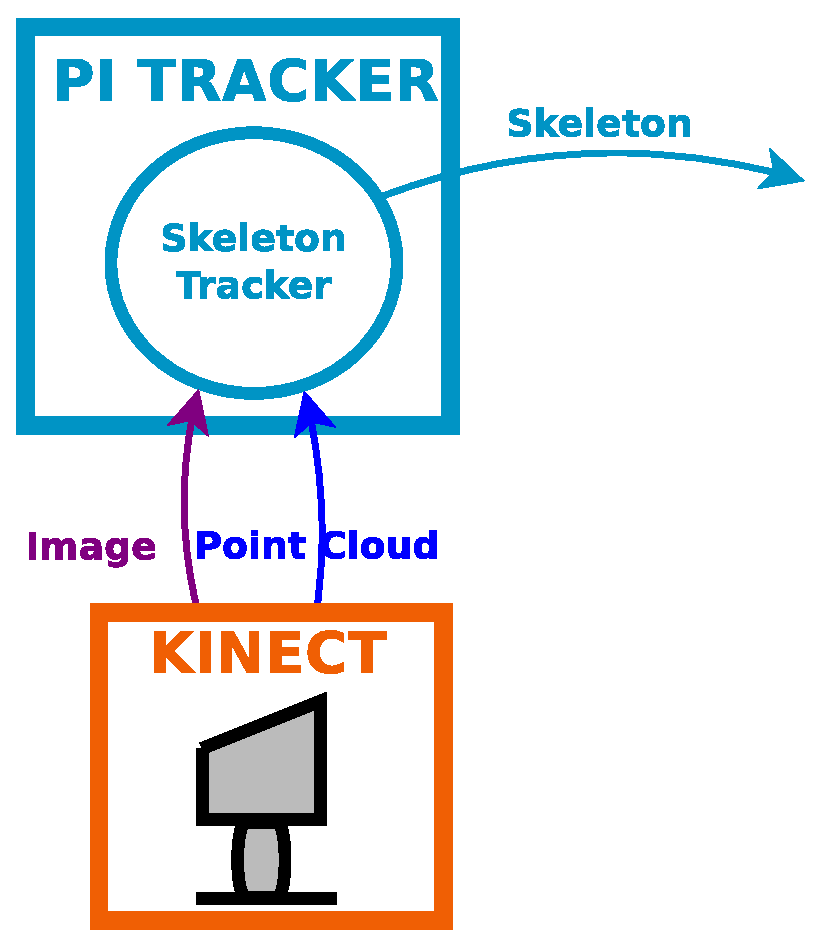
\includegraphics[width=0.3\linewidth]{img/diagrams/node_pi_tracker.eps}
			\caption[Skeleton Tracker I/O]{Connectivity graph of the Skeleton Tracker node.}
			\label{diagram_skeleton}
			\end{center}
		\end{figure}

It can be seen that the node takes as input the output data of the openni\_launch ROS package. 
The node outputs the Skeleton message in which the positions and orientations of the joints are represented. 



%\newpage
%%%%%%% SOFTWARE NODES %%%%%%
%\addcontentsline{toc}{subsection}{Software nodes}
\subsection{Description of the developed nodes}
\label{nodes}


The processing of the system is divided in nodes. 
Figure \ref{nodes_graph} shows the graph of the nodes that have been developed for the project.
% First the ones using the raw input data to the system and afterwards the ones that deliver the output of the system are described.
The circles represent the nodes. %Each circle is a node and the name inside them is the one being used in the software. 
The arrows show the communication between nodes. 
The names next to the nodes' interconnections are the messages interchanged.  % that those processes interchange. 
% The squares with the names serve as separators of the different packages that are being used. 
The square areas define the different ROS packages that have been used.
The square with the tile "OCULAR" separates the nodes developed in this thesis from third-party nodes. 
% All the nodes inside the square with the title "OCULAR" are the ones I developed. 
Sections \ref{converter} to \ref{last_node} present the processing performed by each node. 
\\


		\begin{figure}[H]
			\begin{center}
			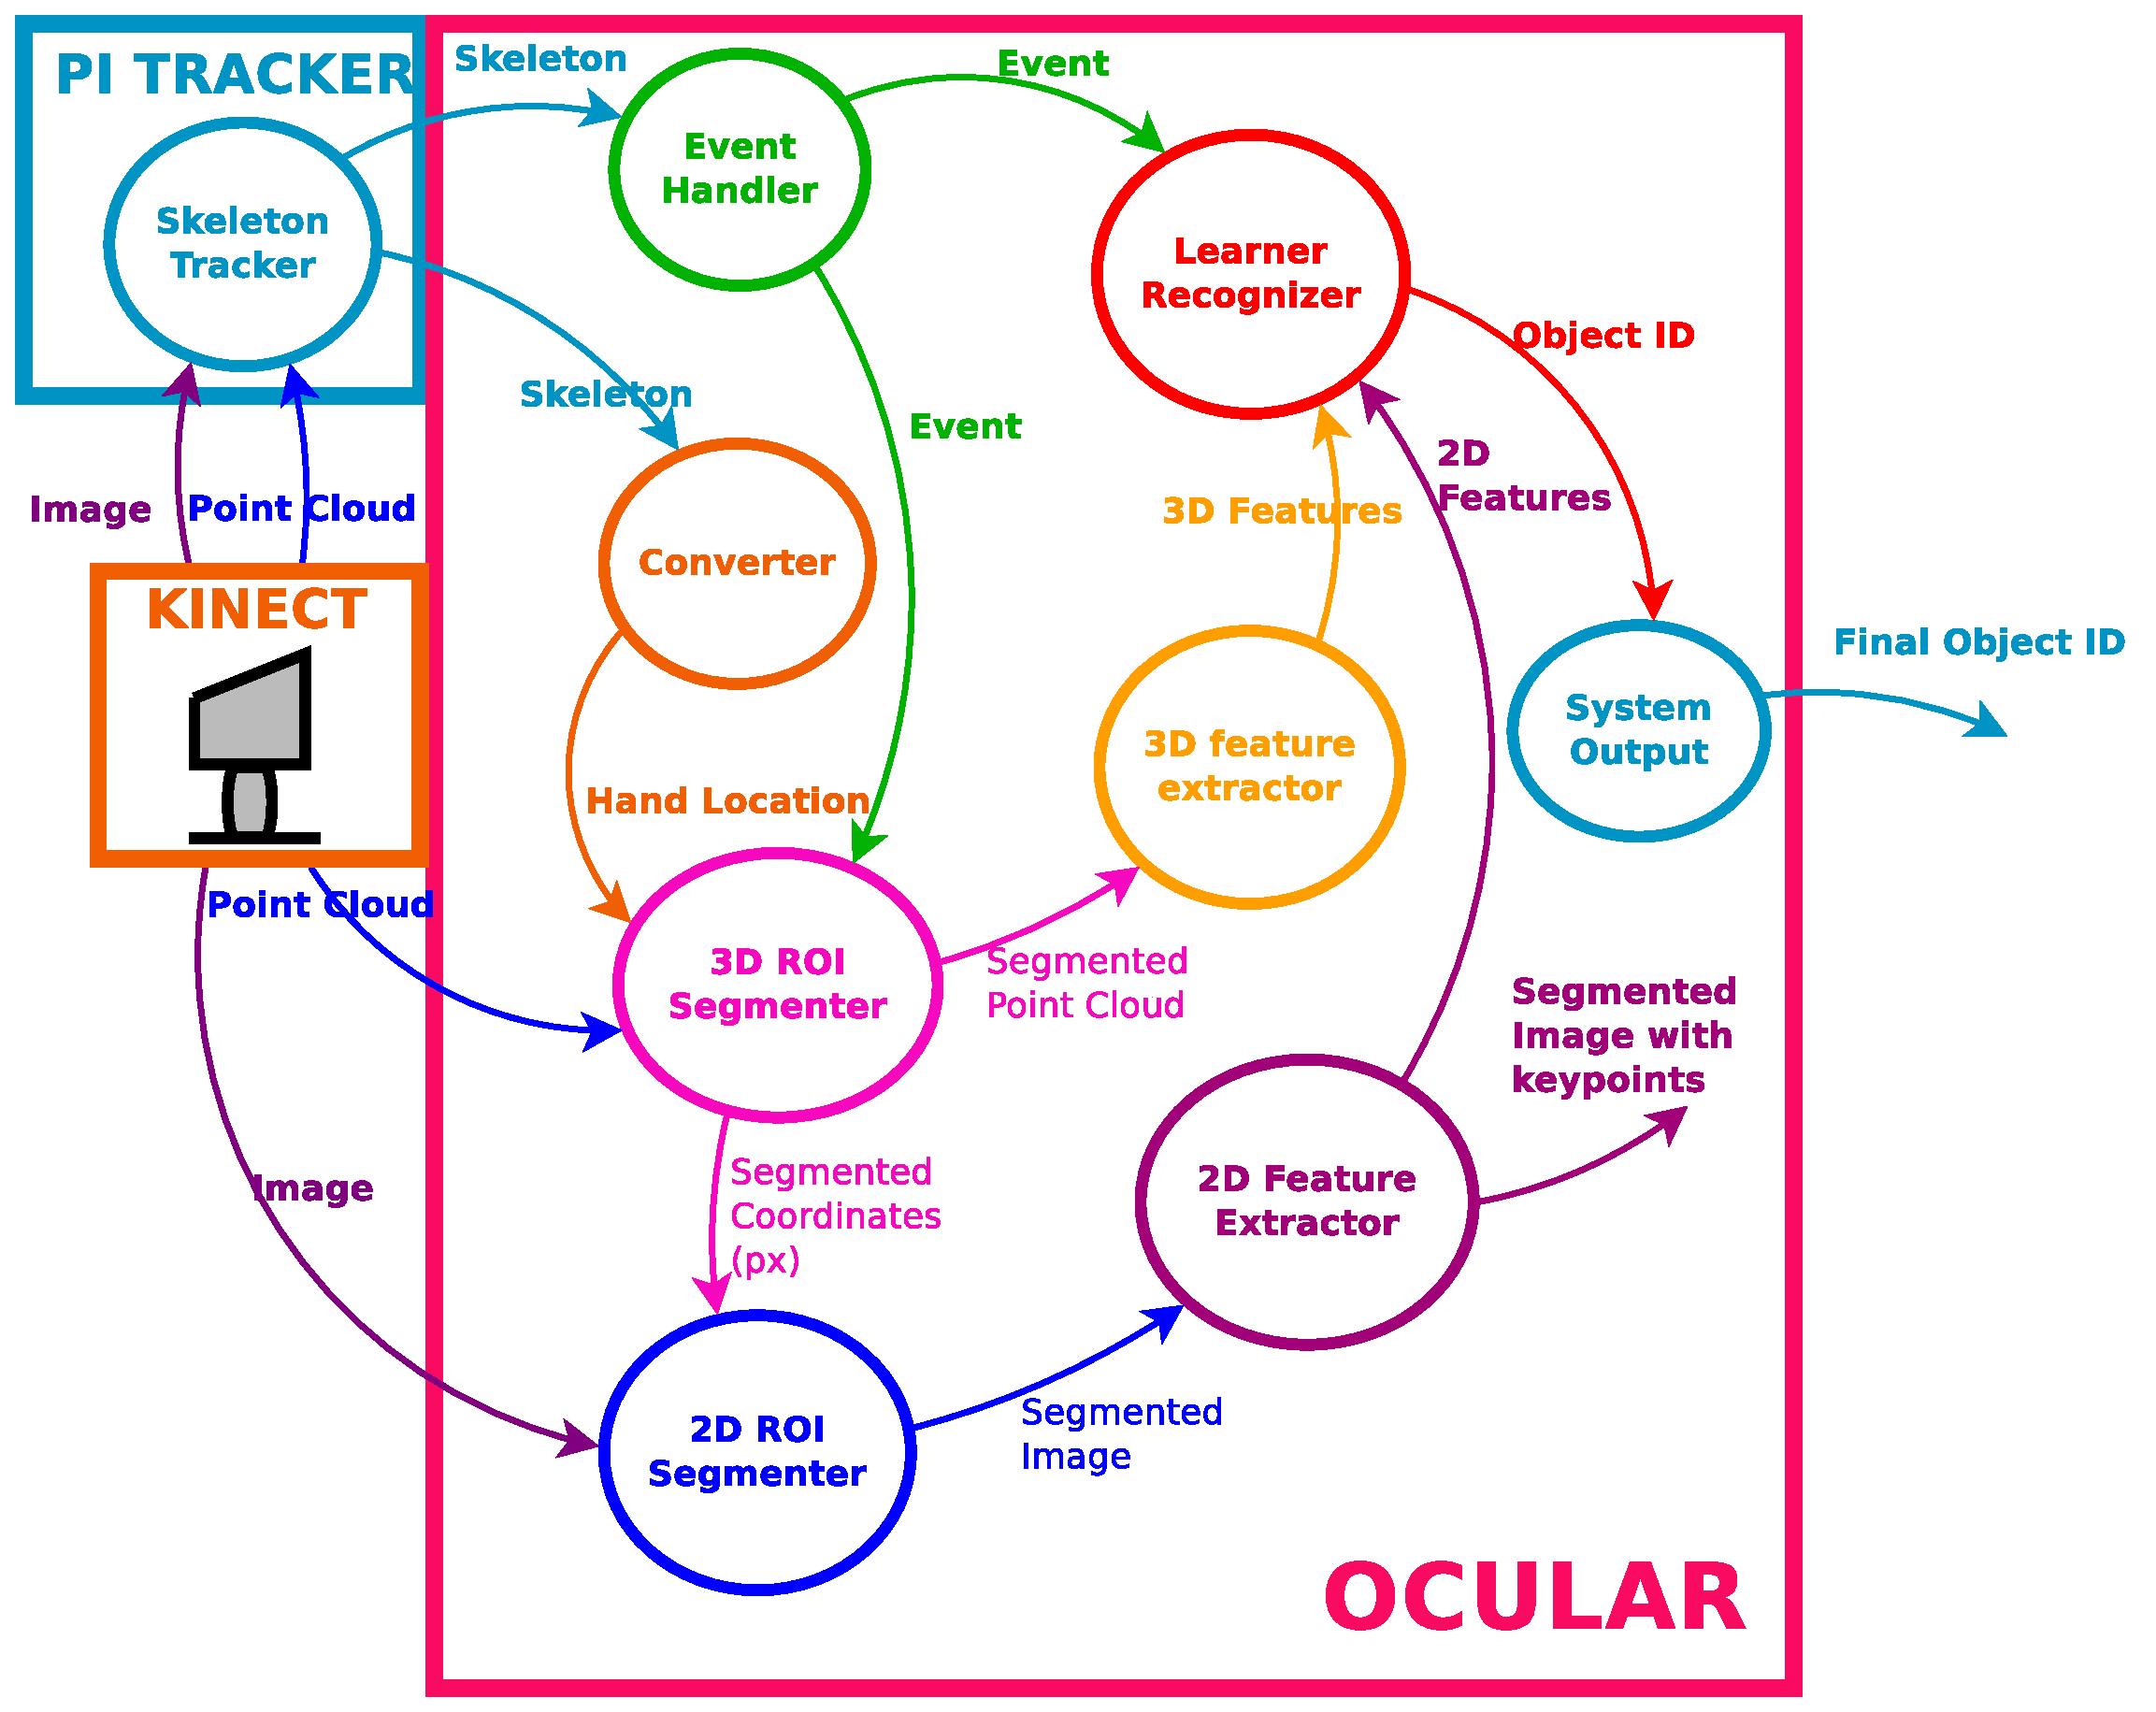
\includegraphics[width=\linewidth]{img/diagrams/nodes.eps}
			\caption[System nodes]{System nodes and their interaction.}
			\label{nodes_graph}

			\end{center}
		\end{figure}

%\newpage



%%\newpage


\subsubsection{Converter node}
		\label{converter}

	This node is the first step of the developed software. 
	It converts the input data containing the skeleton position to a custom message used through the rest of the code. 
	It allows to easily change the package from which the skeleton is obtained without affecting the whole system. 
	The converter node transforms the input data from the pi\_tracker package into the custom message used within the software. 
	It was only implemented a converter for the pi\_tracker package, but it could be easily developed a converter for other packages that retrieve the skeleton position. 
	Figure \ref{node_converter} represents the Connectivity graph of the node. 
	The skeleton message enters the node and the custom message containing the hands location is the output. 

		\begin{figure}[H]
			\begin{center}
			\includegraphics[width=0.5\linewidth]{img/diagrams/node_converter.png}
			\caption[Converter node I/O]{Connectivity graph of the Converter node.}		
			\label{node_converter}
			\end{center}
		\end{figure}

	% The information provided by that third-party code contains the position in the space of each joint of the body. 
	% The converter node takes only both hand's position. 
	The use case diagram of the node can be seen in figure \ref{uc_converter}. 

	\begin{figure}[H]
		\centering
		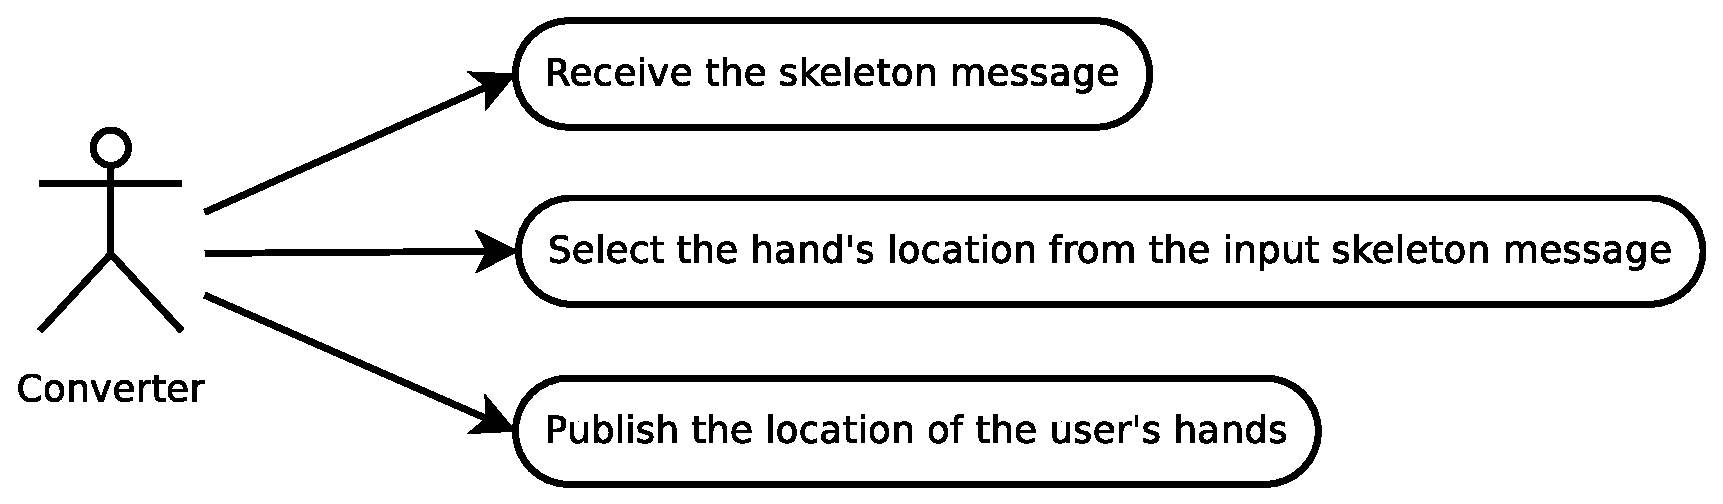
\includegraphics[scale=0.4]{img/diagrams/uc_converter.eps}
		\caption[Use case diagram converter node]{Use Case diagram of the converter node}
		\label{uc_converter}
	\end{figure}

	
	%%\newpage

\subsubsection{3D ROI Segmenter node}
	\label{roi_segmenter_3d}

	Figure  \ref{node_roi3d} presents the Connectivity graph of the node. 
	The input of this node is the raw 3D information from the sensor and the hand's locations from the third-party package pi\_tracker, as well as the hand in which the user is holding the object. 

		\begin{figure}[H]
			\begin{center}
			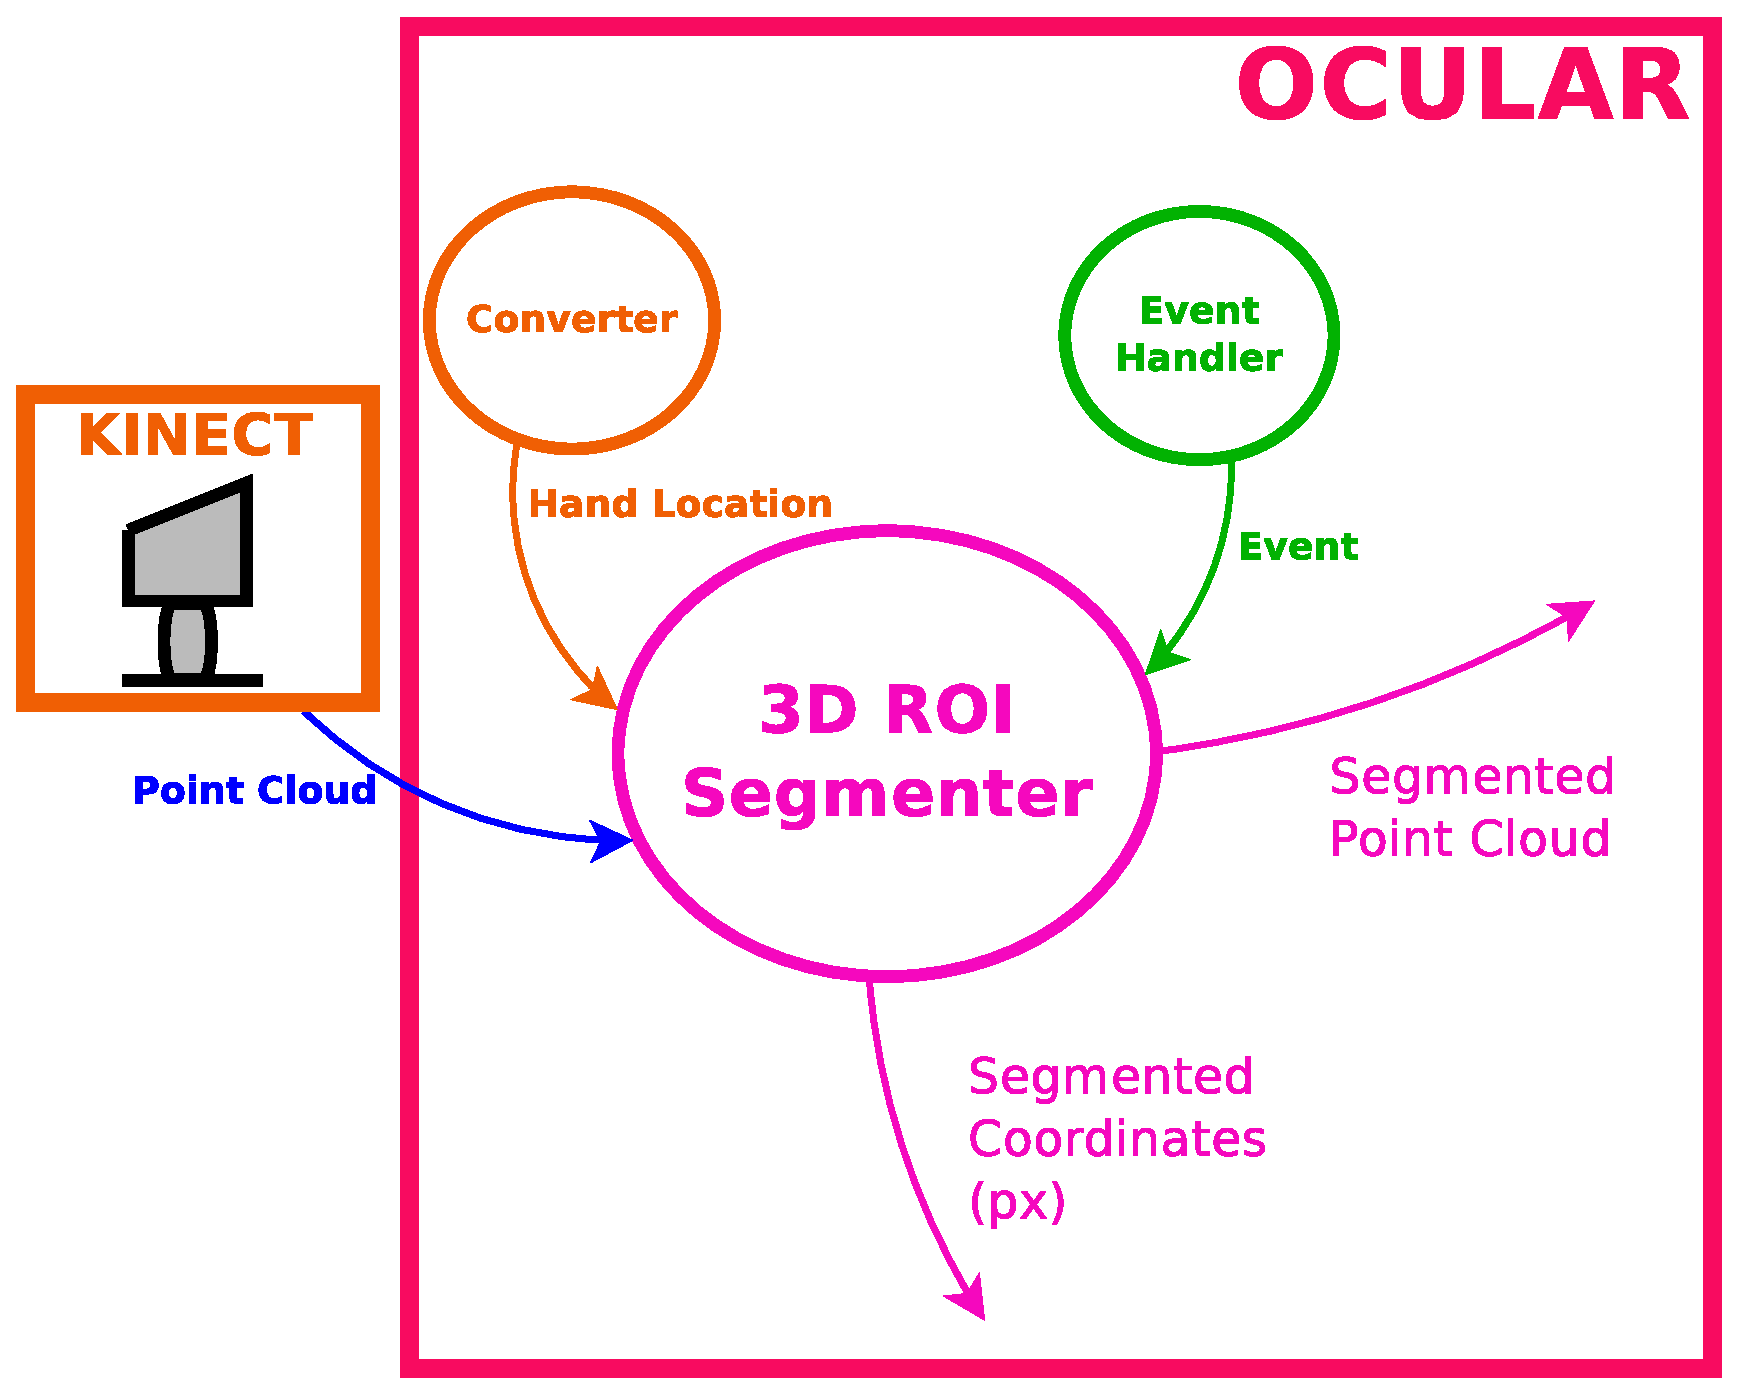
\includegraphics[width=0.5\linewidth]{img/diagrams/node_roi3d.eps}
			\caption[ROI segmenter 3D node I/O]{Connectivity graph of the ROI segmenter 3D node.}		
			\label{node_roi3d}
			\end{center}
		\end{figure}


	The node segments a prism from the original point cloud around the selected hand's center. 
	The prism vertex coordinates are transformed from world coordinates to pixels. 
	This is done to allow the ROI Segmenter 2D to perform the cropping of the input image using those pixel values. 
	That information is the output of the node, together with the segmented point cloud. 
	Figure \ref{uc_roi3d} shows the use case diagram of the node. 

	\begin{figure}[H]
		\centering
	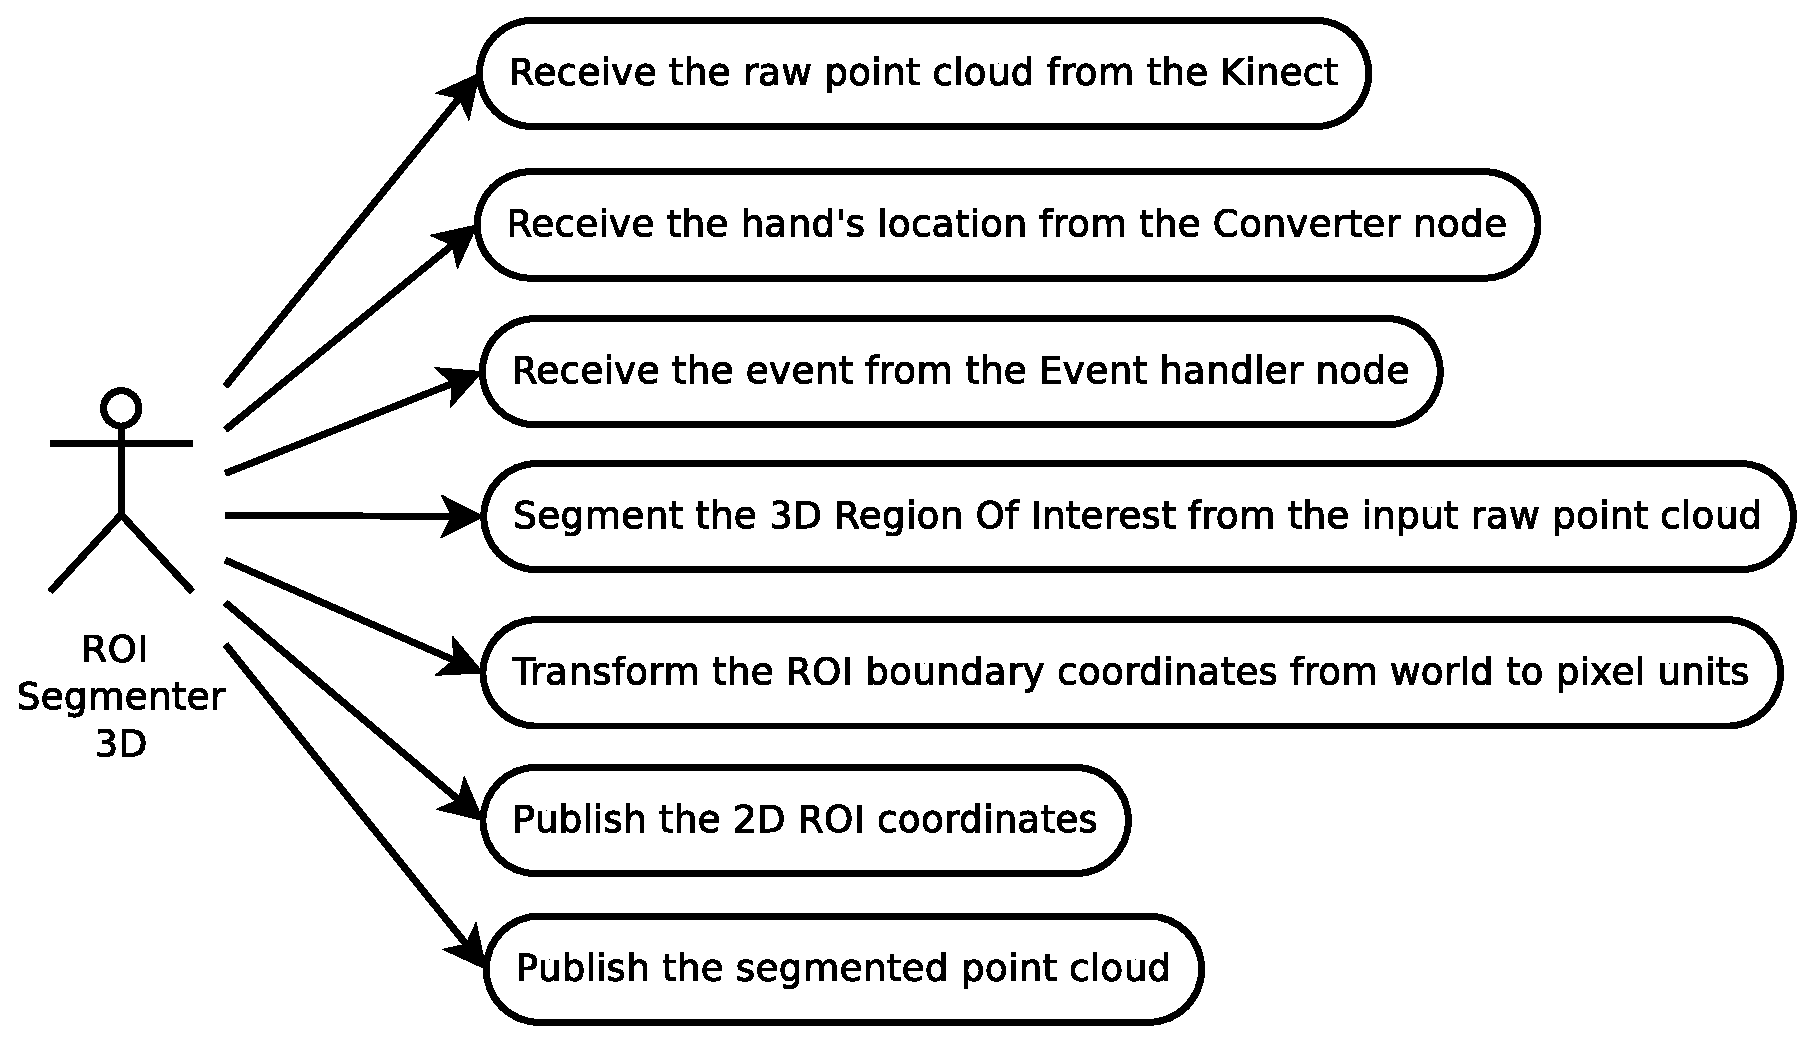
\includegraphics[scale=0.4]{img/diagrams/uc_roi_segmenter_3d.eps}
		\caption[Use case diagram ROI segmenter 3D node]{Use Case diagram of the ROI segmenter 3D node}
		\label{uc_roi3d}	
	\end{figure}
 
%%\newpage

\subsubsection{2D ROI Segmenter node}
	\label{roi_segmenter_2d}
	
	%The present node takes as the input the raw 2D information from the RGB-D sensor and the hand's locations in pixels returned from the ROI segmenter 3D node. 
	Figure \ref{node_roi2d} depicts the Connectivity graph of this node. 
	The raw 2D information and the hand location in pixels are inputs to the ROI Segmenter 2D node. 

		\begin{figure}[H]
			\begin{center}
			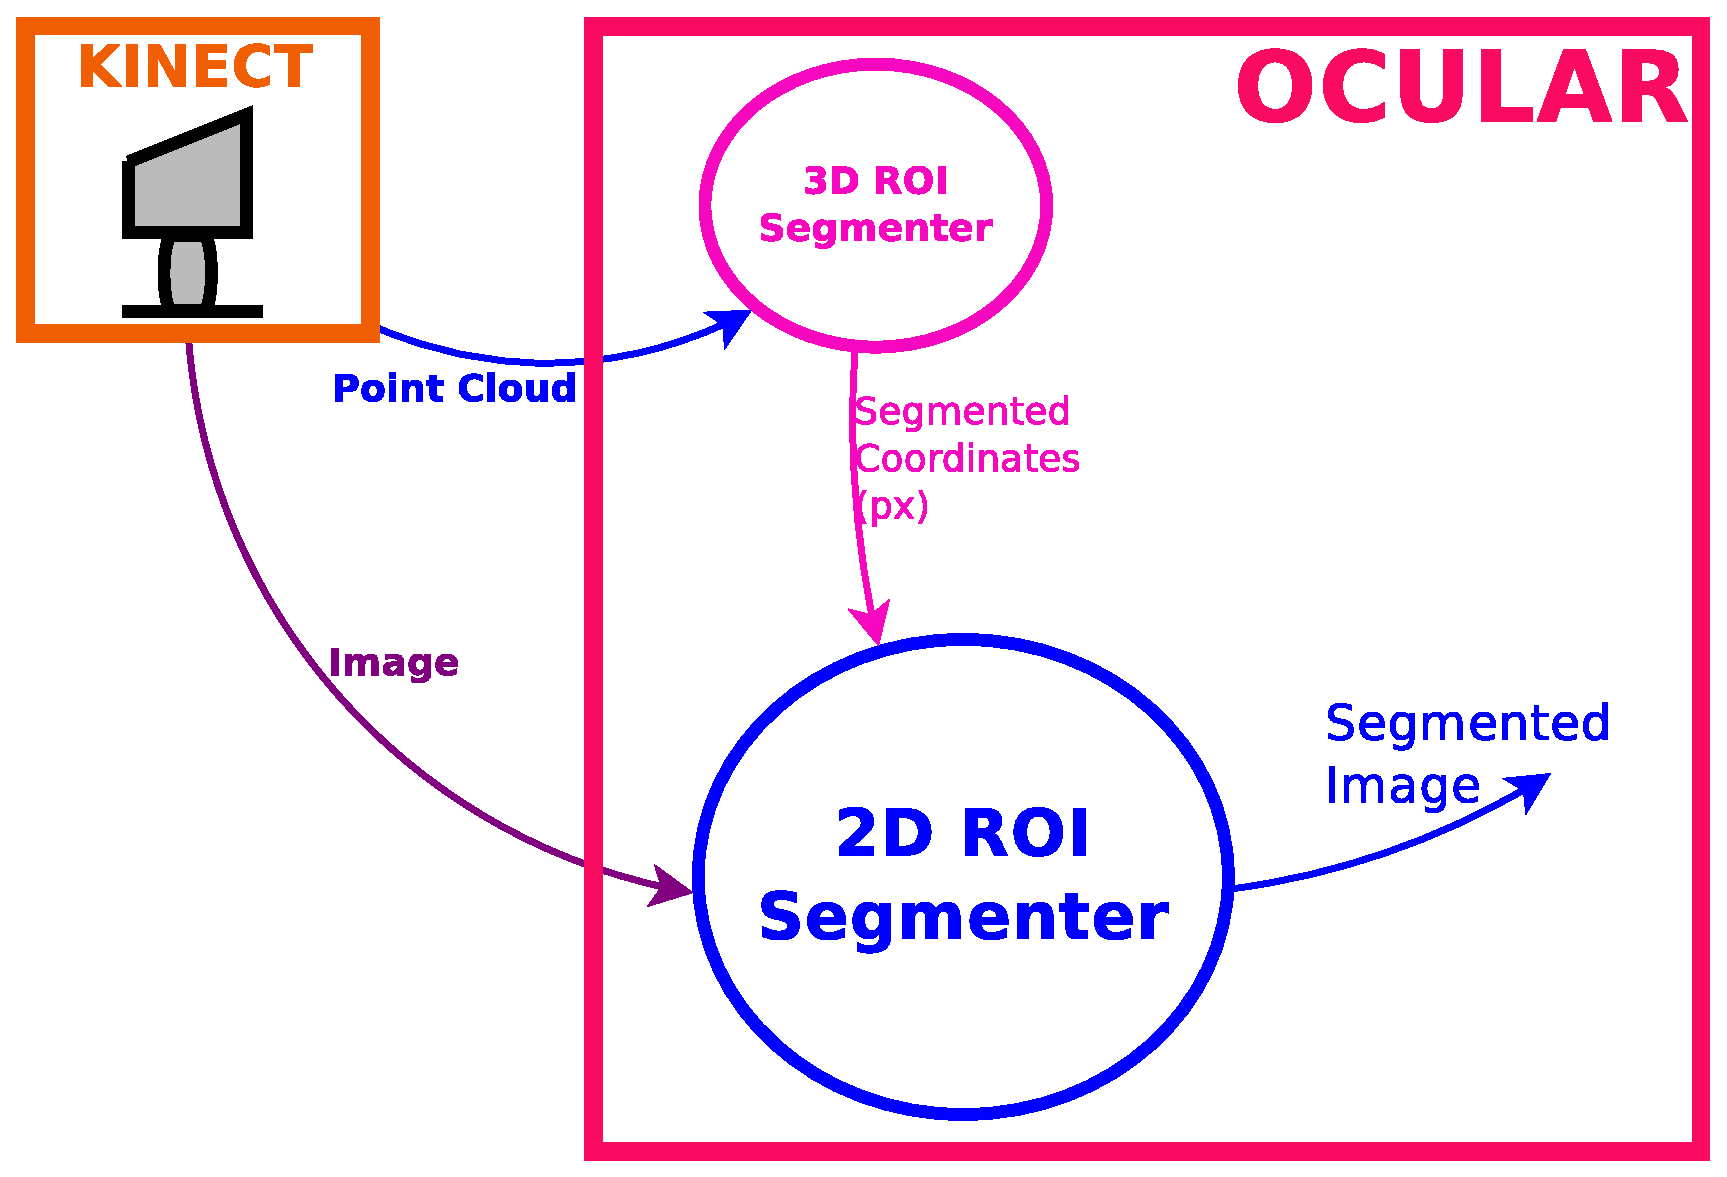
\includegraphics[width=0.5\linewidth]{img/diagrams/node_roi2d.eps}
			\caption[ROI segmenter 2D node I/O]{Connectivity graph of the ROI segmenter 2D node.}		
			\label{node_roi2d}
			\end{center}
		\end{figure}

	The processing performed is the following: First, the ROI (Region Of Interest) is cropped taking a square section around the center of the hand. 
	The size of that figure is fixed for simplicity. 
	This fact does not affect the segmentation since the difference in the scale in negligible in the operating range of the system. 
	The range is determined by the skeleton tracker node and also the low resolution of the RGB-D sensor. 
	The system may be used at a distance between 1.5m and 2.5m. 
	%Since due to the RGB-D sensor's current resolutions the user must remain at a fixed distance from the sensor, the difference in the scale due to the distance is negligible and hence the size can be fixed. 
	\\
	In figure \ref{uc_roi2d} the use case diagram of the node can be observed.
	\begin{figure}[H]
		\centering
			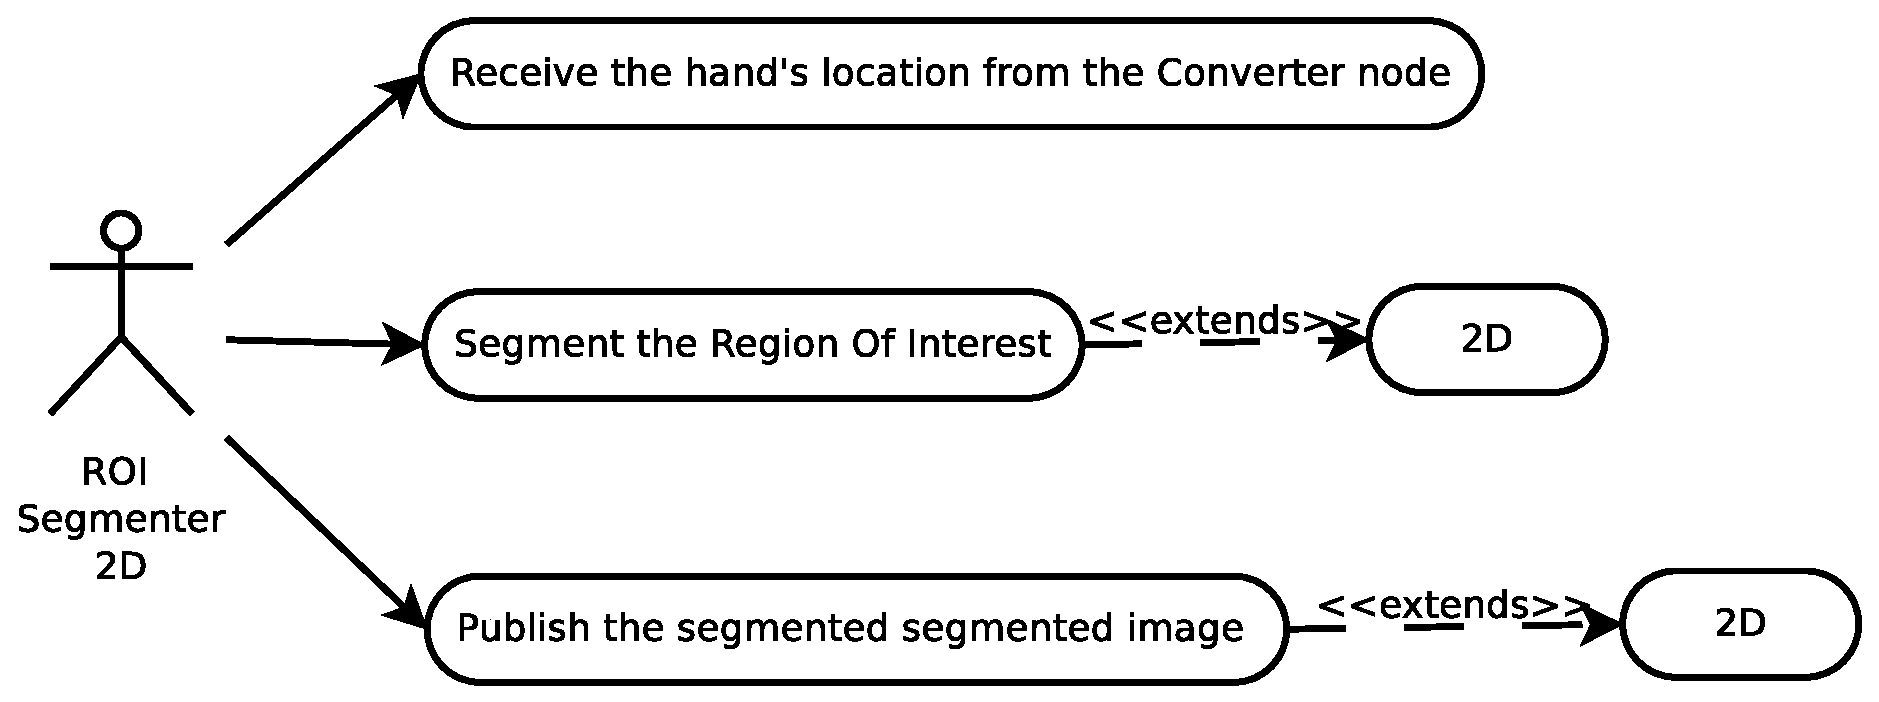
\includegraphics[scale=0.4]{img/diagrams/uc_roi_segmenter_2d.eps}
			\caption[Use case diagram ROI segmenter 2D node]{Use Case diagram of the ROI segmenter 2D node}
		\label{uc_roi2d}
	\end{figure}

%%\newpage

\subsubsection{2D Feature Extractor node}

	This node takes as an input the segmented 2D ROI from the previous nodes and extracts the features. 
	Figure \ref{node_fe2d} shows the Connectivity graph of the node. 

		\begin{figure}[H]
			\begin{center}
			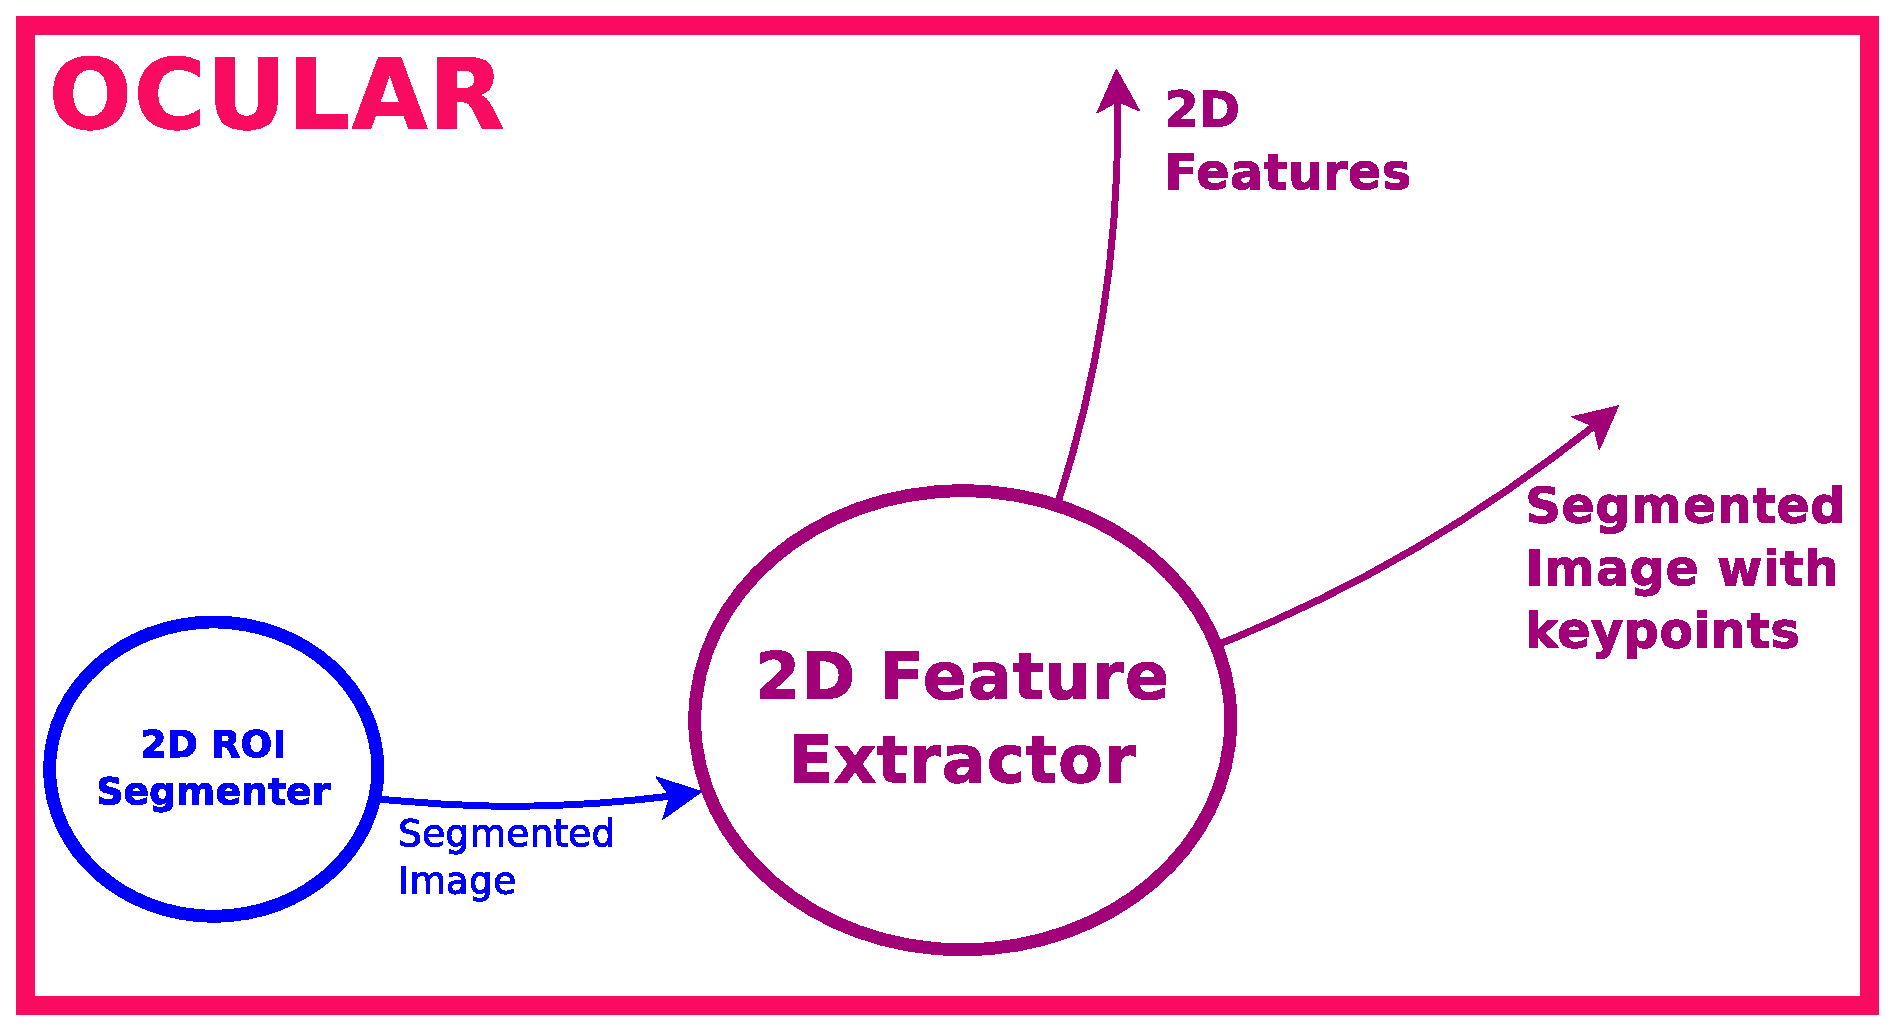
\includegraphics[width=0.5\linewidth]{img/diagrams/node_fe2d.eps}
			\caption[Feature Extractor 2D node I/O]{Connectivity graph of the Feature Extractor 2D node.}		
			\label{node_fe2d}
			\end{center}
		\end{figure}

	There are two output messages of this node, the segmented images with keypoints and the 2D ORB descriptors. 
	The descriptors matrix is the one being used in the rest of the system. 
	The segmented image with the keypoints drawn on it is outputted for debugging and development reasons. 
	\\

	Figure  \ref{uc_fe2d} represents the use case diagram of this node. 
	\begin{figure}[H]
		\centering
			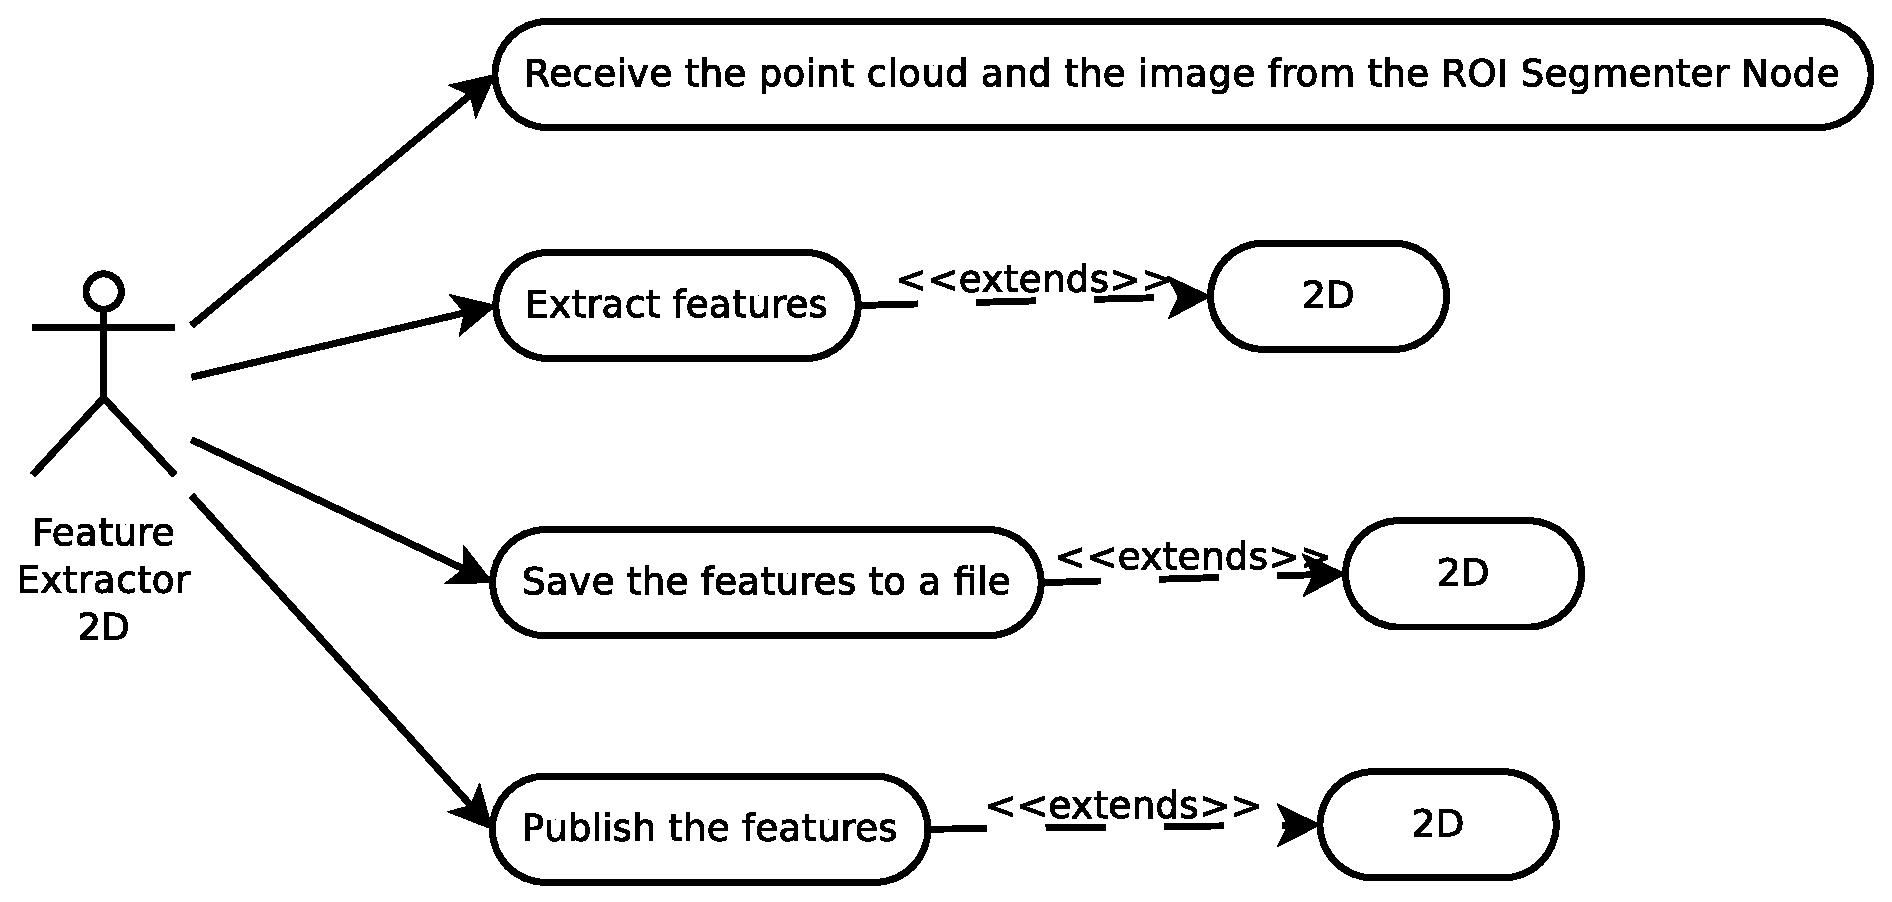
\includegraphics[scale=0.4]{img/diagrams/uc_feature_extractor_2d.eps}
			\caption[Use case diagram Feature Extractor 2D node]{Use Case diagram of the Feature Extractor 2D node}
		\label{uc_fe2d}
	\end{figure}

%%\newpage

\subsubsection{3D Feature Extractor node}

	The input of this node is the segmented point cloud from the ROI Segmenter 3D node (see section \ref{roi_segmenter_3d}. The descriptors are extracted from this information and are published in the output topic. 
	\\
		\begin{figure}[H]
			\begin{center}
			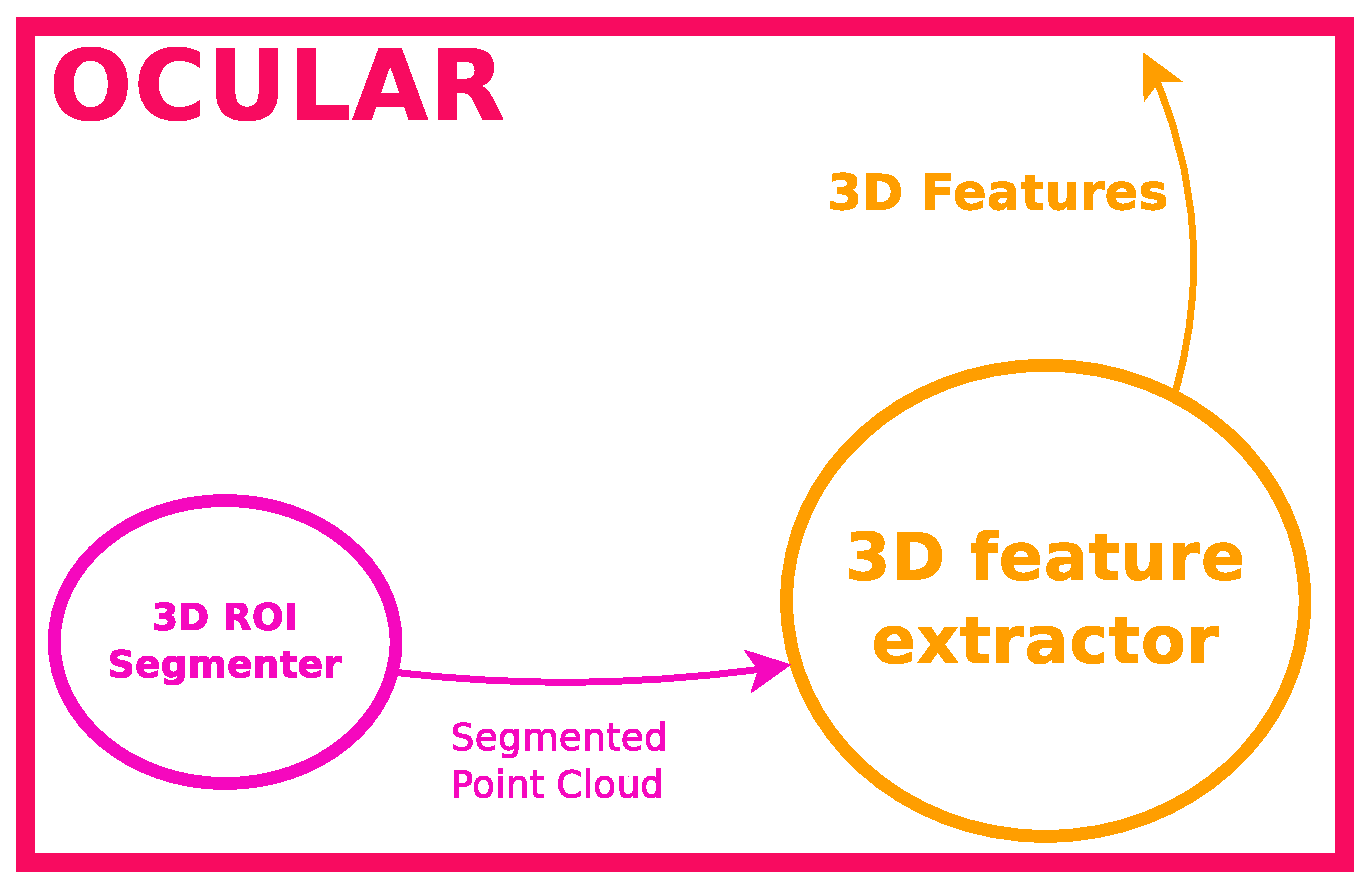
\includegraphics[width=0.5\linewidth]{img/diagrams/node_fe3d.eps}
			\caption[Feature Extractor 3D node I/O]{Connectivity graph of the Feature Extractor 3D node.}		
			\label{node_fe3d}
			\end{center}
		\end{figure}

	Figure \ref{uc_fe3d} shows the use case diagram of the node. 

	\begin{figure}[H]
		\centering
			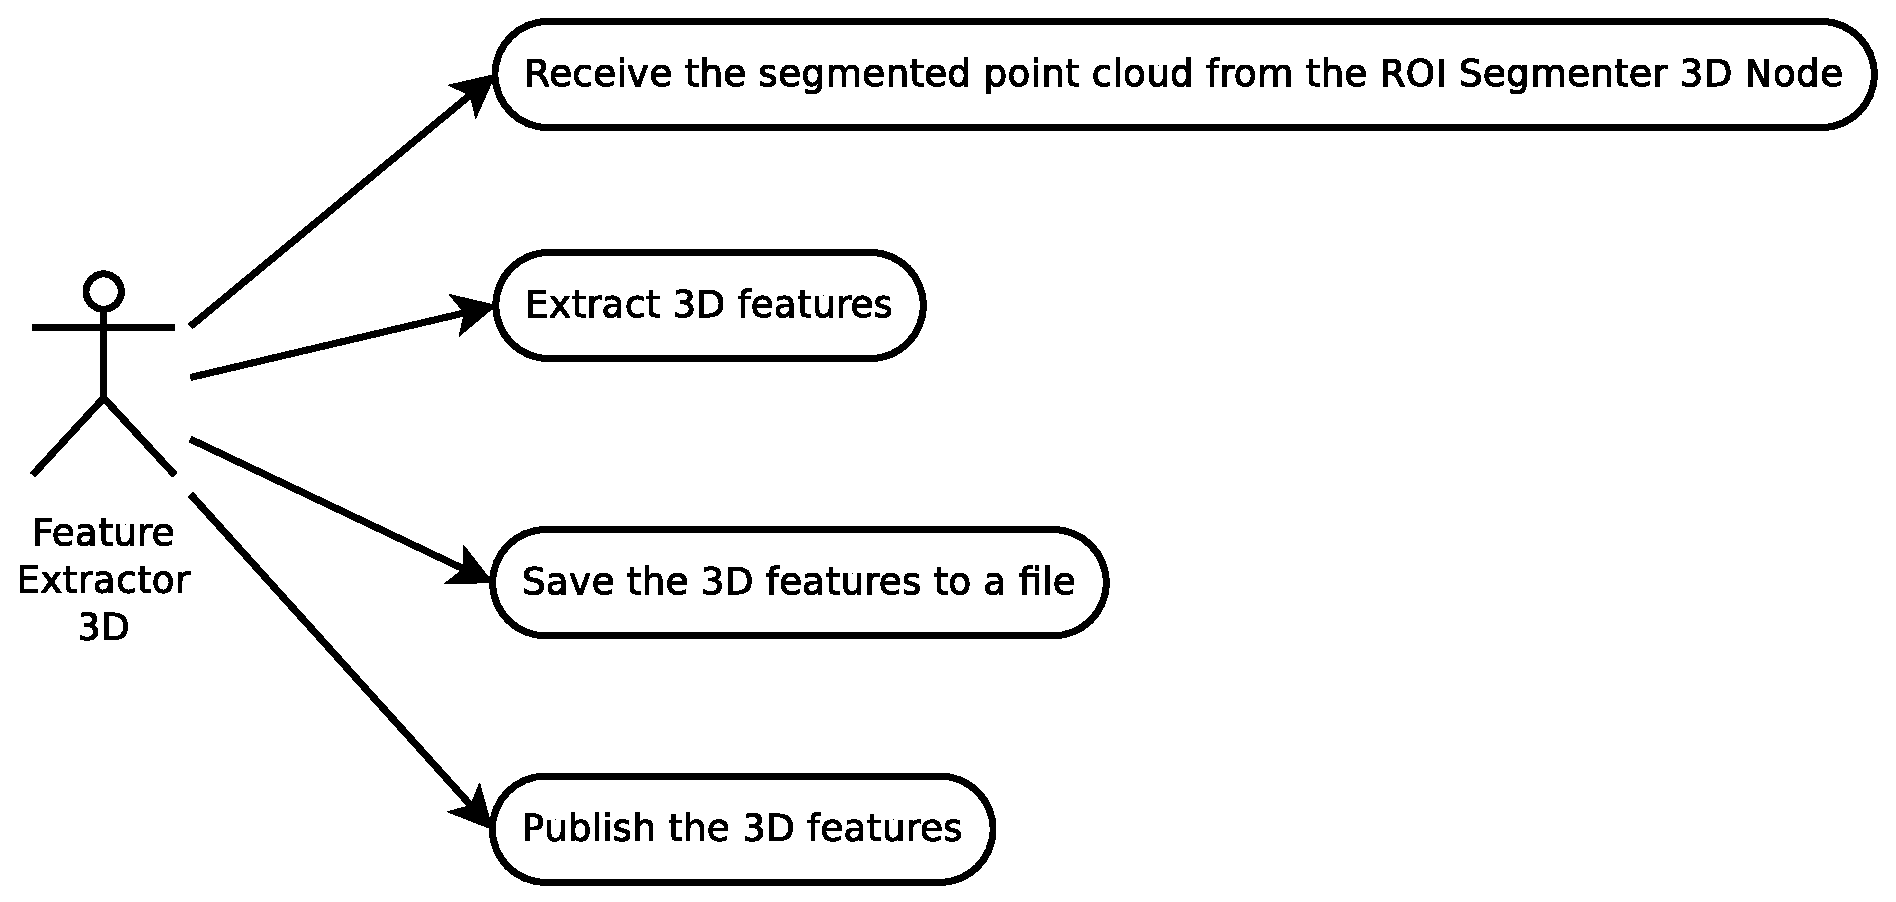
\includegraphics[scale=0.4]{img/diagrams/uc_feature_extractor_3d.eps}
			\caption[Use case diagram Feature Extractor 3D node]{Use Case diagram of the Feature Extractor 3D node}
		\label{uc_fe3d}
	\end{figure}

%%\newpage

\subsubsection{Event Handler node}

	As it was previously stated, in order to interact with the software some gestures were defined. This is the module that detects those gestures and switches accordingly to the corresponding event. This is the node responsible of detecting the different events that can appear in the system. 
	\\
	Figure \ref{node_event} shows the different Connectivity graph of the node. 
		\begin{figure}[H]
			\begin{center}
			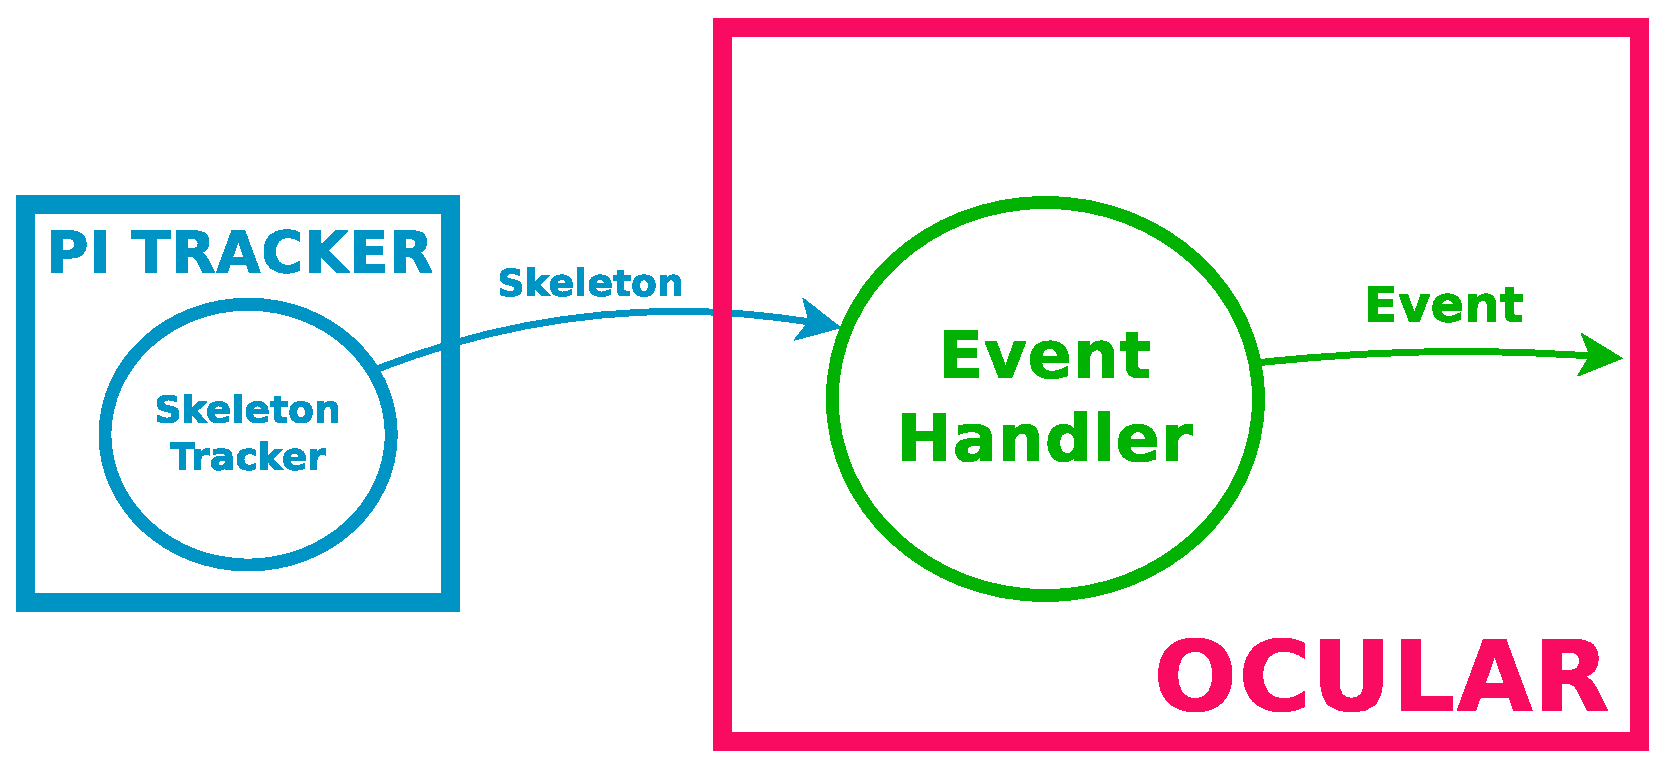
\includegraphics[width=0.5\linewidth]{img/diagrams/node_event.eps}
			\caption[Event Handler 3D node I/O]{Connectivity graph of the Event Handler node.}		
			\label{node_event}
			\end{center}
		\end{figure}
	The input of the system is the skeleton message that is obtained from the third-party package pi\_tracker. This message contains the information of all the joints of the user. The information is screened to detect the height at which each hand is located. The one that is the highest is the one being used in the software. Afterwards, the distance between the body and the chosen hand is computed. When that distance is similar to the distance of the user's arm, the event triggered is "learn". If, otherwise, the hand is located close to the body, the event that is published to the output topic is "recognize". 
	\\

	The distance that triggers the modes is proportional to the distance between the user and the RGB-D sensor in order to obtain a range of use of the software higher. 
	Figure \ref{uc_event} is a diagram with the use case of the node. 
	\begin{figure}[H]
		\centering
			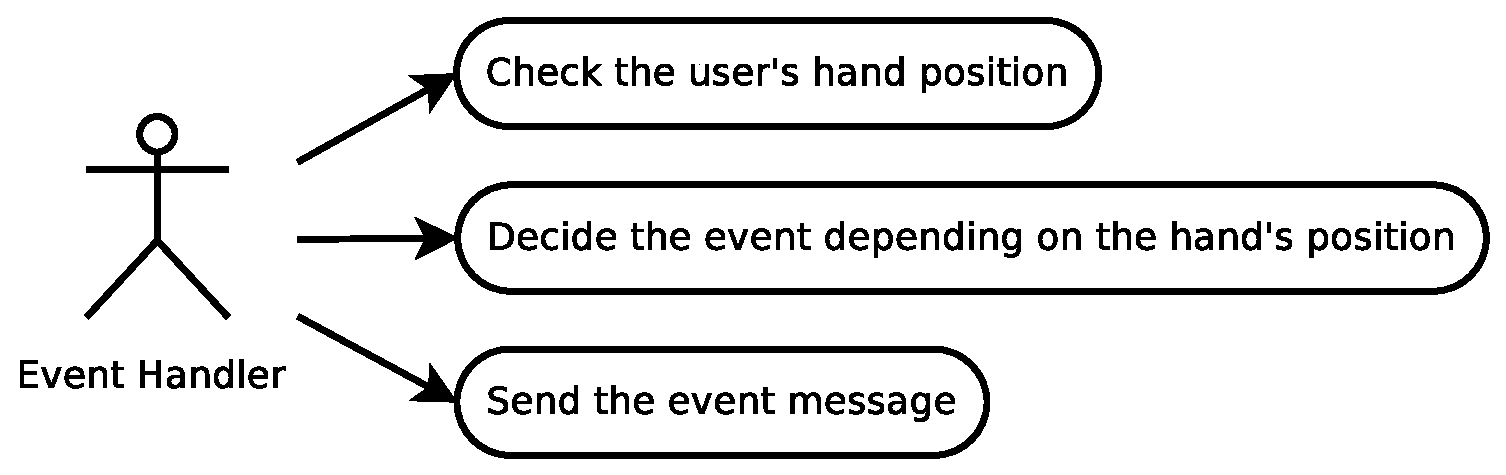
\includegraphics[scale=0.4]{img/diagrams/uc_event_handler.eps}
			\caption[Use case diagram Event Handler node]{Use Case diagram of the Event Handler node}
		\label{uc_event}
	\end{figure}

%%\newpage

\subsubsection{Learner-Recognizer node}
\label{learner_recognizer}

	This node implements the state machine depending on the events recognized by the event handler node. If the event received is "learn", the learning sequence starts. If the event is "recognize", the recognize sequence is triggered. 
	\\

		\begin{figure}[H]
			\begin{center}
			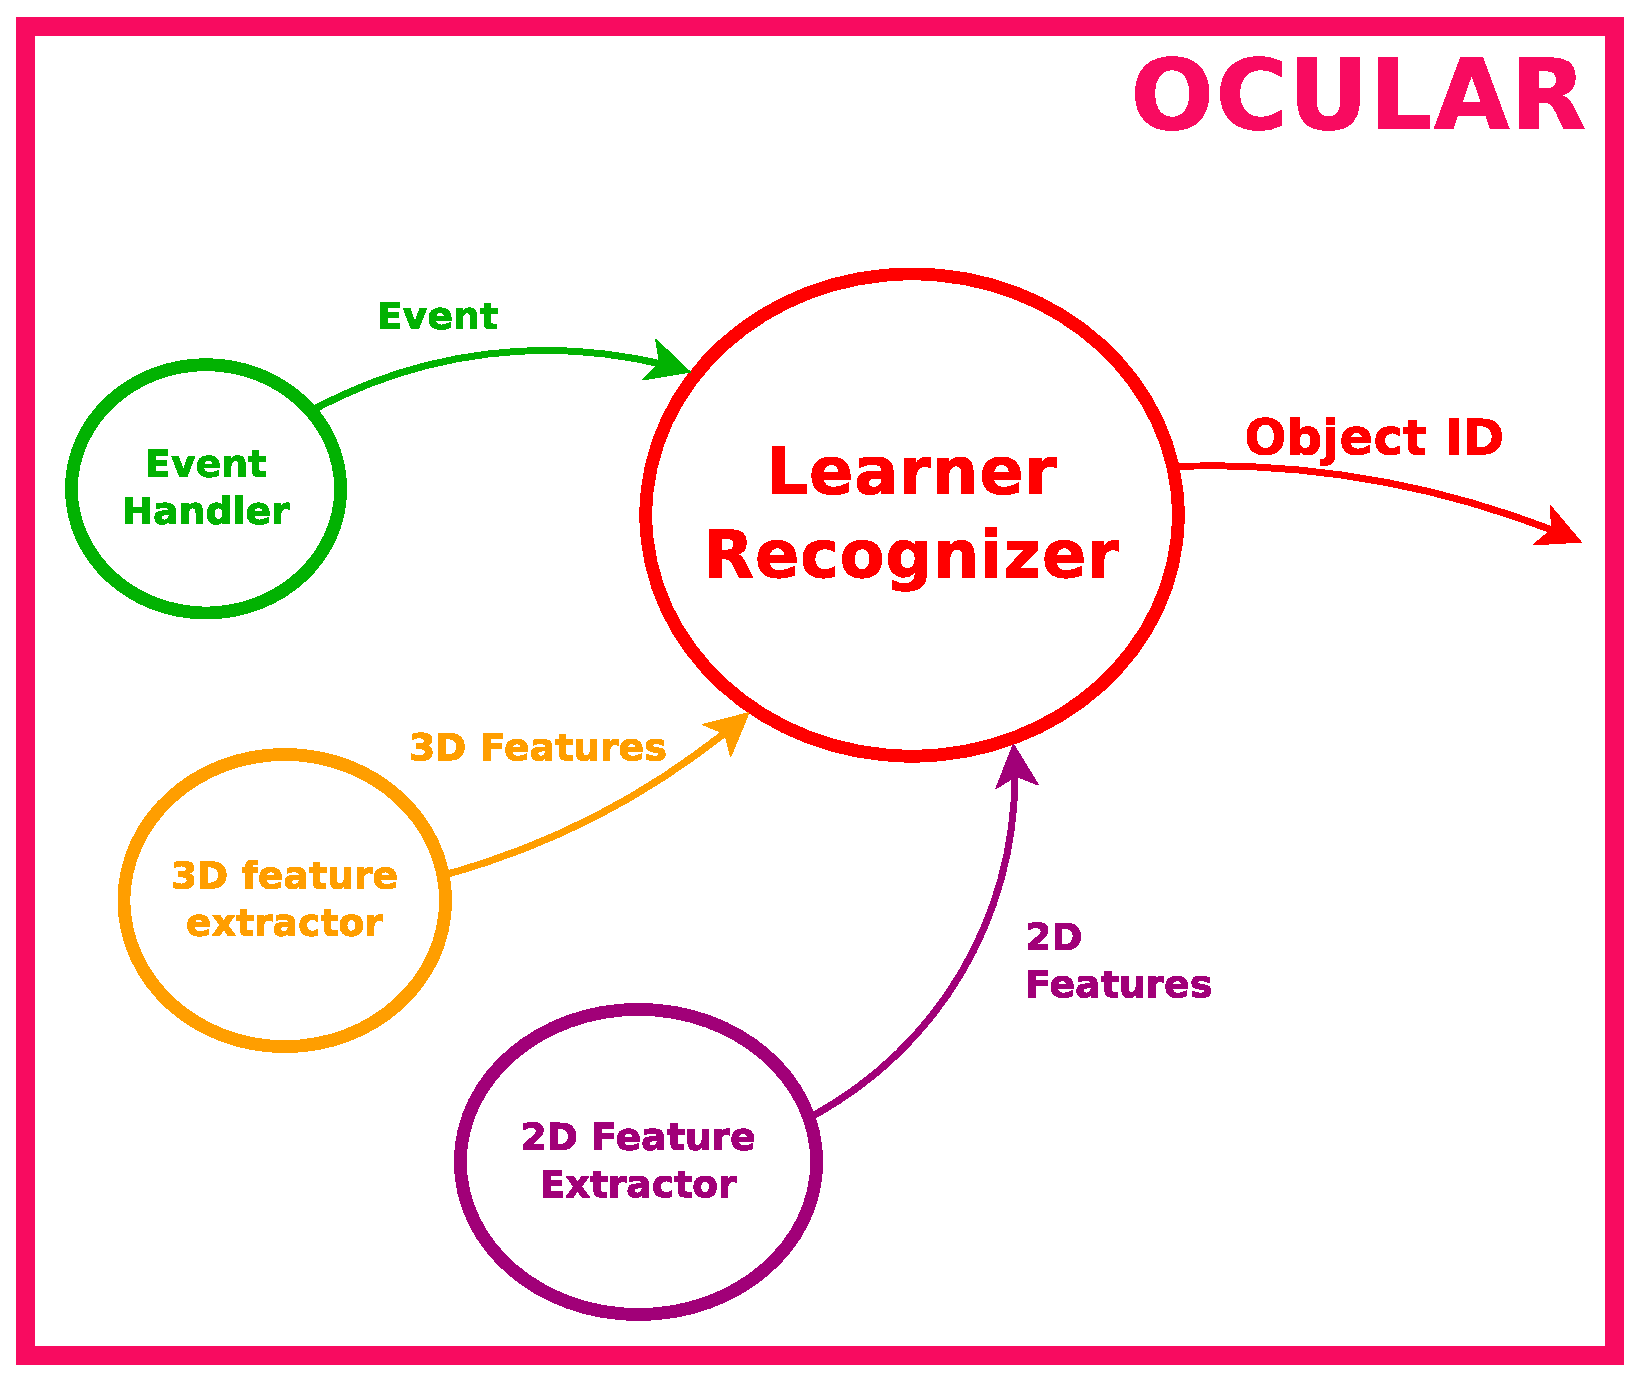
\includegraphics[width=0.5\linewidth]{img/diagrams/node_lr.eps}
			\caption[Learner-Recognizer node I/O]{Connectivity graph of the Learner-Recognizer node.}		
			\end{center}
						\label{node_lr}

		\end{figure}

	The learn sequence consists in obtaining and storing the features both 2D and 3D and waiting a second allowing the user to move the object to capture a new view of it. 
	The dataset extracted is saved to a folder when the software is closed, to prevent possible lags in the runtime of the program. 
	Each view is saved separately. 
	This node loads the files that are still in the saving folder when the program is restarted. 
	\\

	The recognition sequence compares the newly obtained features both 2D and 3D with the ones that are stored in the dataset. 
	Afterwards, the result of the recognition for both types of descriptors are published in the output topic. 
	Figure \ref{uc_learner_recognizer} presents the use case diagram of the node. 

	\begin{figure}[H]
		\centering
			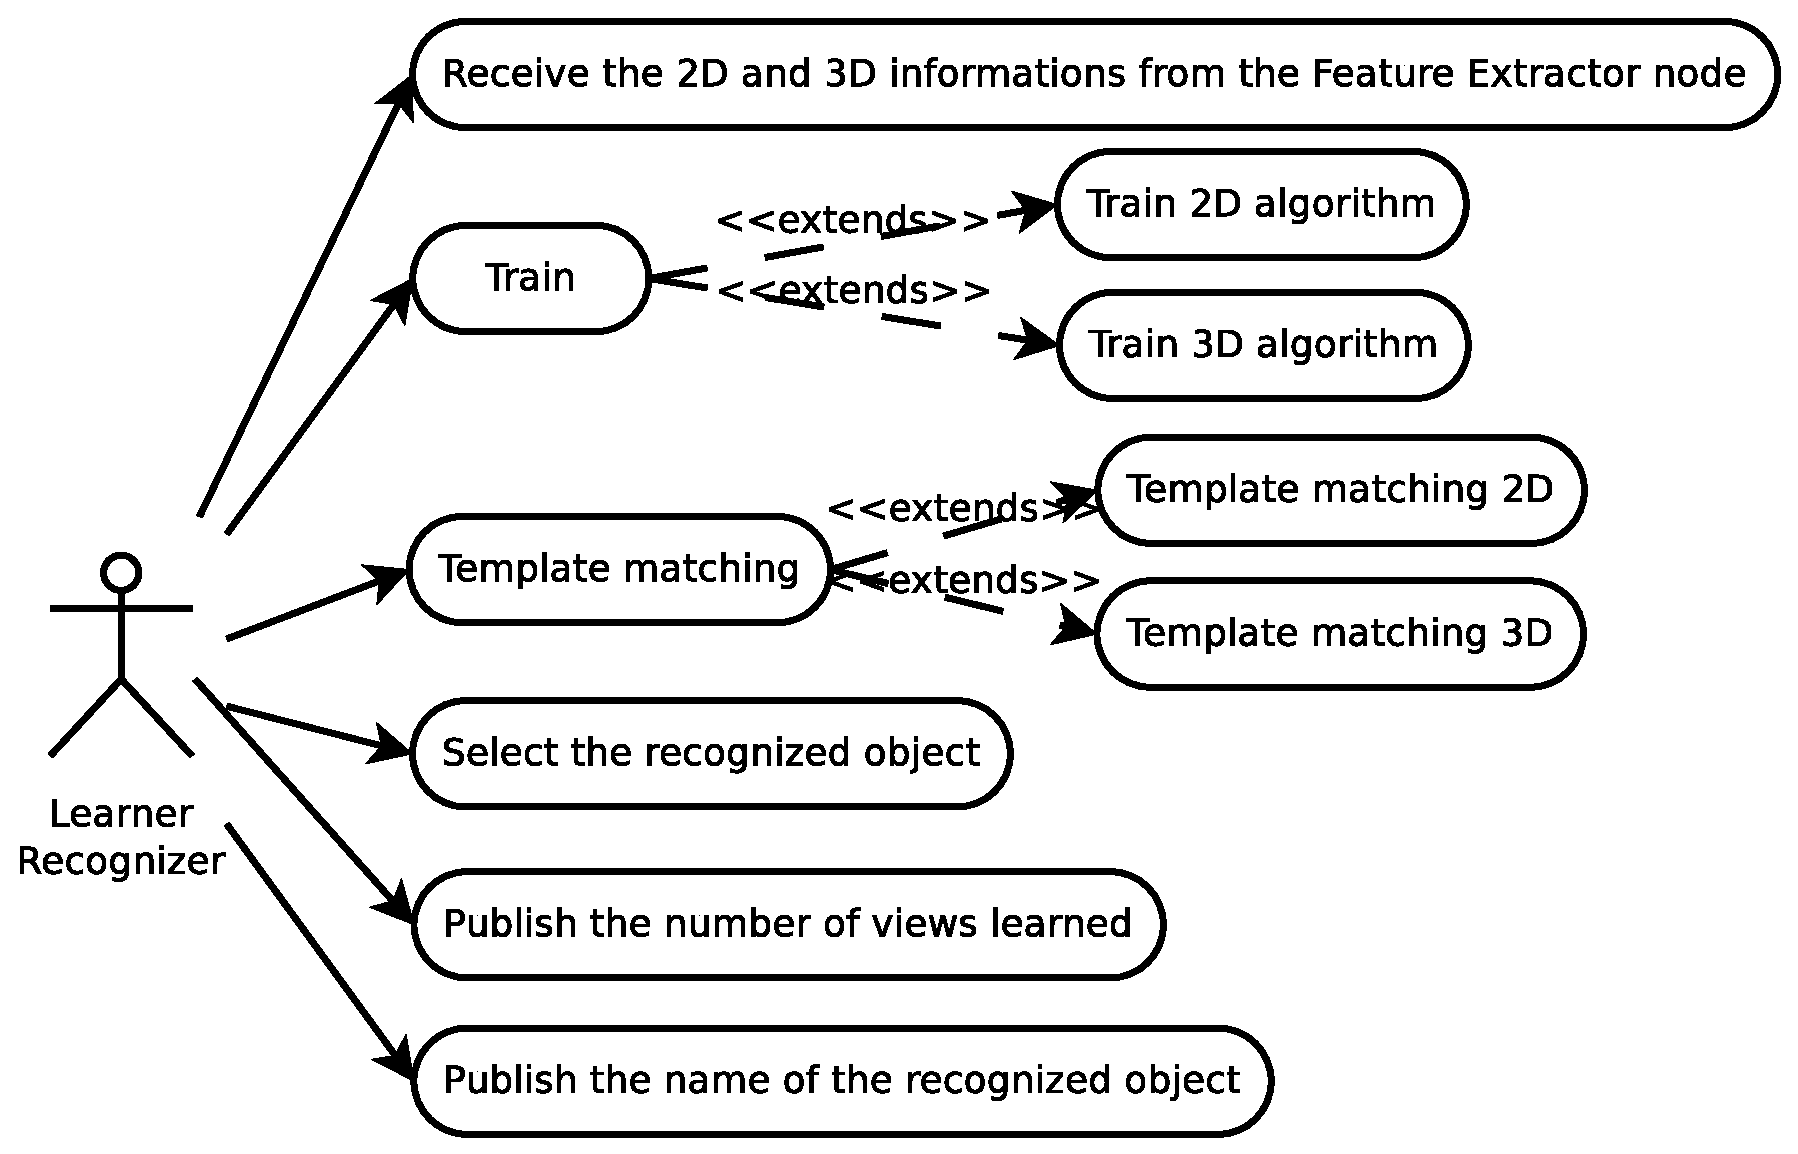
\includegraphics[scale=0.4]{img/diagrams/uc_learner_recognizer.eps}
			\caption[Use case diagram Learner-Recognizer node]{Use Case diagram of the Learner-Recognizer node}
			\label{uc_learner_recognizer}
	\end{figure}

%%\newpage


\subsubsection{System Output node}
\label{last_node}
	This nodes implements a buffer and a decision algorithm. 
	The input of the node is the object ID message from the Learner-Recognizer process as can be seen in figure \ref{node_output}.
	The node stores thirty values of instantaneous object estimations. 
	Since the Kinect runs at 30 frames per second, each second a new final object estimation appears. 
	The output of the node is the final object ID. 


		\begin{figure}[H]
			\begin{center}
			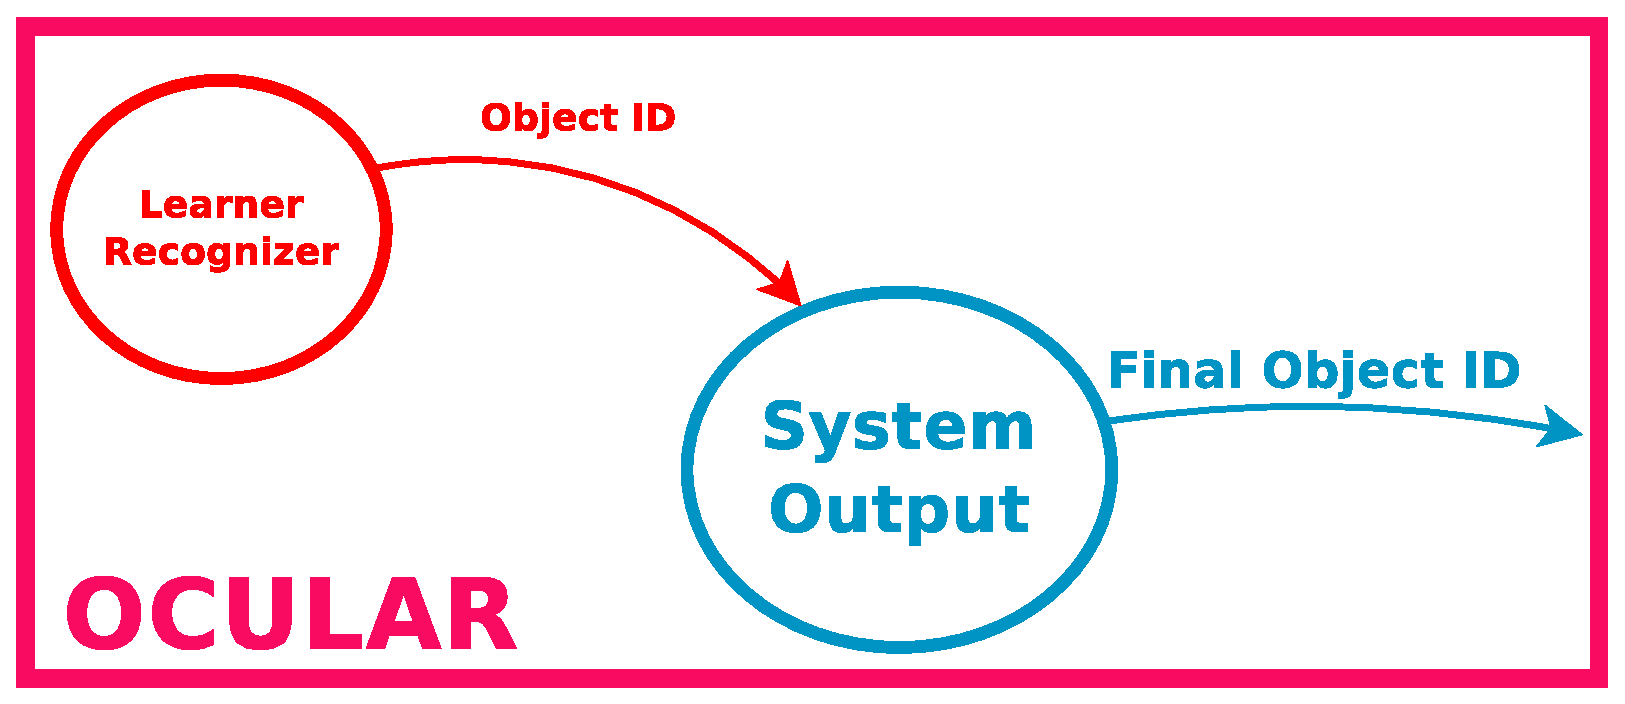
\includegraphics[width=0.5\linewidth]{img/diagrams/node_output.eps}
			\caption[System Output node I/O]{Connectivity graph of the System Output node.}		
			\label{node_output}
			\end{center}
		\end{figure}

	The decision is performed as follows. 
	The input to the algorithm are two vectors containing the 2D and 3D object estimations. 
	The frequency of each class is obtained. 
	Let us represent as $y'_{2D}$ and $y'_{3D}$ the vectors containing in each element the frequency of the object with $object_id = element$. 
	Both informations are combined in one vector called $y'$. 
	\\
	\begin{center}
	$y'=0.6*y'_{2D}+0.4*y'_{3D}$
	\end{center}
	More importance is being given to the 2D estimations since the 2D descriptors are more robust than the 3D ones. 
	The estimated final object id ($Y$) is obtained as the vector element that has the highest value. 
	\\
	\begin{center}
		$Y'= argmax(y')$
	\end{center} 
	This number $Y$ is the output of this whole system. 
	\\
	Figure \ref{uc_output} shows the use case diagram of this node. 

	\begin{figure}[H]
		\centering
			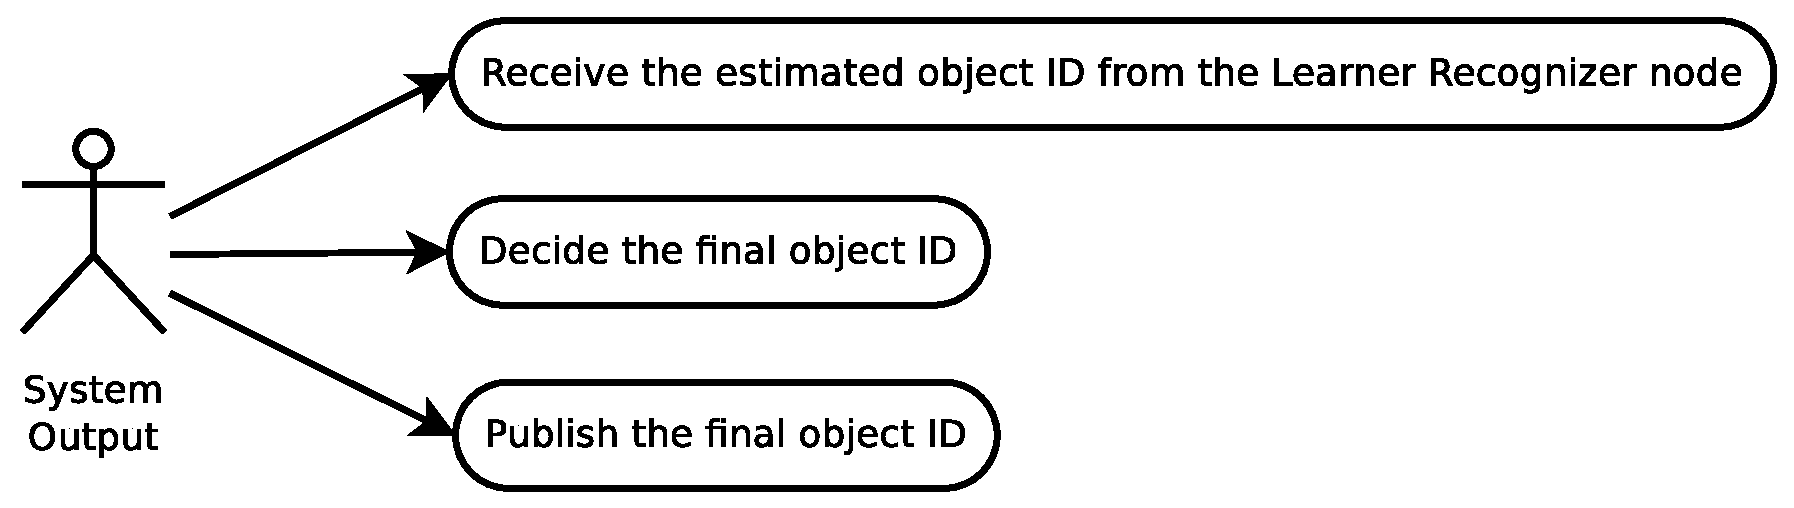
\includegraphics[scale=0.4]{img/diagrams/uc_system_output.eps}
			\caption[Use case diagram System Output node]{Use Case diagram of the System Output node}
			\label{uc_output}
	\end{figure}
 
\newpage
\section{Software topics}
\label{software_topics}

The topics are the channels that communicate the nodes in the ROS framework. All the nodes in the software are constantly obtaining messages from the input topics and publishing the results of their computation to the output ones. 
\\

In this section a relation of all the topics used in the software is presented. 


\subsection{Hand location}
The complete path of this node in the code is: /TFG/CONVERTER/hand\_location. The messages published in this node are the TFG/
\subsection{Event}
This node is filled by the node event\_handler. The message used by this node is the custom message TFG/EventHandler. The full name of this topic is /TFG/EVENTHANDLER/event. 

\subsection{Descriptors 2D}
The complete name is /TFG/FE2D/descriptors2D. In this topic the Feature Extractor 2D node publishes the matrix of descriptors extracted from the segmented image. To this topic the Learner Recognizer node is subscribed in order to obtain those descriptors.  

\subsection{Descriptors 3D}
In this topic the Feature Extractor 3D publishes the descriptors of the segmented point cloud. The Learner Recognizer node is subscribed to it. 
The complete path to the topic is /TFG/FE3D/descriptors3D.


\subsection{/TFG/ROI2D/segmented\_image}
The path  is /TFG/ROI2D/segmented\_image. In this topic the  ROI Segmenter 2D node publishes its output, the image with the region of interest. To this topic the Feature Extractor 2D is subscribed. 


\subsection{/TFG/ROI2D/segmented\_image\_with\_keypoints}
The topic's name is /TFG/ROI2D/segmented\_image\_with\_keypoints. This topic is filled with images showing the segmented 2D ROI with the keypoints drawn on it. The node that publishes this data is FeatureExtractor2D. The topic is intended for visualization and troubleshooting purposes. 

\subsection{/TFG/ROI3D/segmented\_coordinates\_px}
\subsection{/TFG/ROI3D/segmented\_pc}
\subsection{/TFG/object\_id}

\newpage
\subsection{Messages}
\label{messages}

In this section the custom messages used within the software are explained. These messages allow an easier communication between nodes providing them with sufficient information to perform each task. 
\\

All messages have a header, that provides basic information such as the exact time at which it was send. 


\subsubsection{EventHandler message}
The structure of this message is as follows: \\

Header header\\
string hand\\
string event\\
string last\_event

\\

It is the message used within the event topic. Provides information about the hand the user is utilizing in the software, the event that is currently occurring and the last event that was produced. 
\\

The inclusion of the last event provides information about the changes in the events, allowing the software to recognize the different combinations that can appear and act accordingly. 
\\

That decision mechanism is implemented in the learner\_recognizer node. 

\subsubsection{HandImage message}

The HandImage message has the following structure: \\
Header header\\
string[] name\\
sensor\_msgs/Image[] image

This message only differs on the image standard message on the appearance of a name and on the vectorial nature of its attributes. It is intended to serve on future expansions of the code in which for each hand a different action is performed. 

\subsubsection{HandLoc message}
This message has the following structure: 
Header header\\
int32 user\_id\\
string[] name\\
geometry\_msgs/Vector3[] position
\\

It contains the information of the absolute position of the hand and its name. It is as well vectorial, that is the same message variable can store multiple informations that are accessed as the C arrays. 

\subsubsection{HandLocPx message}
The handlocpx message is as follows: 

Header header\\
int32 user\_id\\
string[] name\\
int32[] points\\

As it can be seen is almost identical to the previous message. It only differs on the units in which the hand location is given. in the previous one it was given in meters and in this one, it is in pixels. 
\\

This message is filled by the ROI segmenter 3D node, who transforms the limits of the ROI in meters to pixels for the ROI segmenter 2D note to use. This latter subscribes to the topic in which the message is published and crops the raw input message accordingly. 

% \newpage
% \subsection{Usage}
\label{usage}

In the present section the compilation and installation instructions of the software are presented as well as the usage instructions. 

\subsubsection{Operating System}
This project uses the ROS framework to compile and run. Since ROS is only available for Linux OS, this type of operating system should be installed in the computer used to run the code. 


\subsubsection{Software needed}
In order to use the software developed in this bachelor's thesis, the following packages are needed. 
\subsubsection{ROS}
The Robotic Operating System is used within the software as the means of communication between the different nodes. Also, different ROS packages are used to provide the input information to the system. Hence, it is needed to install it. 
\\

The code has been tested with the Groovy or Indigo ROS distributions. For installation instructions the webpage http://ros.org provide numerous tutorials. 
\\

Between those distributions there is another one which is called Hydro. For this particular one the code has not been tested but since there are no major changes between Hydro and Indigo, the code used for this latter should compile without problems. 


\subsubsection{ROS package: openni\_camera / freenect\_camera}
These packages are the drivers of the kinect. They should be installed via command-line, which is the recommended, or downloading and compiling the source code. 
\\

In order to install these packages using the terminal, please introduce the following commands: 
\\

sudo apt-get install ros-<distro>-openni\_camera
\\

sudo apt-get install ros-<distro>-freenect\_camera
\\

Replace the <distro> word by the distribution currently installed on your computer, Groovy or Indigo, in lower case. 



\subsubsection{ROS package: openni\_launch / freenect\_launch}
These package needs to be launched in parallel with the code provided in this bachelor's thesis. As the previous ones, they can be downloaded using the terminal or compiling the source code. 
\\

In oder to install them using the command-line please enter the following on it: 
\\

sudo apt-get install ros-<distro>-openni\_launch
\\

sudo apt-get install ros-<distro>-freenect\_launch
\\

This commands install the ROS package in the default directory in which the ROS libraries are stored, usually /opt/ros/<distro>. 



\subsubsection{ROS package: pi\_tracker}
The pi\_tracker package is needed in order to retrieve the position of the user's skeleton. Unfortunately it is not available for command-line installing. This means that the code must be downloaded and compiled in order to be used. 
\\

To do so, the source code must be downloaded into the ROS workspace already created. The source code might be found on the web-page: http://github.com/pi\_tracker. 
\\

For further details on how to download and install ROS packages using the source code please read the following section. 

\subsection{ROS packages source code compilation}
The first thing needed is the ROS workspace. Depending on the ROS distribution, this workspace might be a catkin workspace or a rosbuild workspace. 
\\

Catkin and rosbuild are two methods implemented by ROS to organize the code and to compile it. Both use CMAKE below to compile the code, with specific arguments for different compilation options. 
\\

\subsubsection{Catkin workspace}
The first thing needed is to create a folder for the workspace and a src folder within the first one. This can be done through the interface or using the following command in a terminal: 
\\

mkdir -p <path-to-workspace>/<name-of-workspace>/src\\

Then, insert the following command or open a terminal inside the src folder: \\

cd <path-to-workspace>/<name-of-workspace>/src\\

Finally, in order to initiate the catkin workspace, type: \\

catkin\_init\_workspace\\

This creates an empty workspace. The different packages must be located inside the src folder. \\

In order to build the workspace, move to the upper folder of your workspace and insert the following command: \\

catkin\_make\\

This compiles all the packages within the catkin workspace. In order to use the packages inside this folder, it is necessary to source the setup bash files inside the devel folder. This overlays the workspace on top of your ROS environment. Enter the following command: \\

source <path-to-workspace>/<name-of-workspace>/devel/setup.bash\\




\subsubsection{Rosbuild workspace}
First, introduce the following command in order to create the workspace folder: \\

mkdir -p <path-to-workspace>/<name-of-workspace> \\

Then, in order to create the workspace the rosws command is needed, which is not installed by default. It can be downloaded using the Ubuntu package manager introducing the following in a terminal: \\

sudo apt-get install python-rosinstall\\

Now it is possible to create the workspace using: \\

rosws init <path-to-workspace>/<name-of-workspace> /opt/ros/<ROS-distro>\\

In a rosbuild workspace the packages are located within the sandbox folder. To create it and set it insert the following: \\

mkdir <path-to-workspace>/<name-of-workspace>/sandbox\\

rosws set  <path-to-workspace>/<name-of-workspace>/sandbox\\

Whenever the entries in the workspace suffer changes, it is necessary to re-source the setup file inside the workspace to make sure the updated ROS\_PACKAGE\_PATH is used. In order to source the workspace introduce this line in a terminal: \\

source <path-to-workspace>/<name-of-workspace>/setup.bash\\




\subsection{OCULAR compilation}
The source code might be found in the repository : http://github.com/irenesanznieto/ocular. There are two branches within that code, one for the Groovy and the other for the Indigo distributions. 
\\




\subsection{Launch files}

\subsection{Run the code}

